%\documentclass[pdftex,12pt,a4paper]{article}
\documentclass[pdftex,12pt,a4paper]{report}


\usepackage[pdftex]{graphicx}
\usepackage[english]{babel}
\usepackage[utf8]{inputenc}
\usepackage{amsmath,amssymb}
\usepackage{graphicx}
\usepackage{caption}
\usepackage{subcaption}
\usepackage{float}
\usepackage{hyperref}
\usepackage{verbatim}
\usepackage{array}
%\usepackage{amssymb}
%\usepackage{algorithm}
\usepackage[titlenumbered,ruled,linesnumbered,algoruled,boxed,lined]{algorithm2e}
\usepackage[noend]{algpseudocode}
\usepackage{stmaryrd}
\usepackage{makeidx}
\usepackage{upgreek}
\usepackage{setspace}
\usepackage{cite}
\usepackage{etoolbox}
\makeatletter
\patchcmd{\@verbatim}
  {\verbatim@font}
  {\verbatim@font\footnotesize}
  {}{}
\makeatother
\usepackage{rotating}

\usepackage{tikz}
\usetikzlibrary{arrows,automata,positioning,intersections}
\usetikzlibrary{shapes,shapes.multipart}
%\usetikzlibrary{quotes,angles}

\onehalfspacing
\newcommand{\HRule}{\rule{\linewidth}{0.5mm}}

\makeindex

\begin{document}

\begin{titlepage}
\begin{center}

% Upper part of the page. The '~' is needed because \\
% only works if a paragraph has started.


%\textsc{\Large Report on the project}\\[0.5cm]

% Title
\HRule \\[0.2cm]
{\Large \bfseries Integrating Conditional Planning and Robust Execution in Human-Robot Interaction \\[0.2cm] }

\HRule \\[0.5cm]

% Author and supervisor
\noindent
\begin{minipage}[t]{0.4\textwidth}
\begin{flushleft} \large
\emph{Candidate:}\\
Valerio Sanelli\\
\end{flushleft}
\end{minipage}%
\begin{minipage}[t]{0.4\textwidth}
\begin{flushright} \large
\emph{Thesis Advisor:} \\
Luca Iocchi
\end{flushright}
\end{minipage}
\\[2cm]

\end{center}
\vfill
\begin{flushleft}

\includegraphics[width=0.5\textwidth]{images/logo.png}
\end{flushleft}


%\let\thefootnote\relax\footnote{\noindent Report submitted in fulfillment of the requirements for the %project of Medical Robotics at Sapienza - University of Rome.}
\end{titlepage}

\newpage
\tableofcontents
\newpage

\chapter{Introduction}
This chapter present the thesis, with motivations and goal of this work
%\section{Planning}
%\subsection{Planners Characteristics/Requirements}
%\begin{enumerate}
%\item  How to handle failures $\shortrightarrow$ Replanning avoiding loops
%\item  How to represent uncertainty $\shortrightarrow$ Probabilistic reasoning
%\item  How to deal with Exogenous Events $\shortrightarrow$ Implicit/Explicit Modelling 
%\item  Hyerarchical Tasks
%\item  Frame Problem: how to represent the fact that things do not arbitrarly changes.
%\item  Qualification problem: how to deal with the things that prevent me from achieving my intendend result (impossibility of list alla preconditions). 
%\item  How to model/deal time (explicit/implicit)
%\item  World-based (STRIPS) vs Plan-based Planner (Partial-order Planning)
%\item  Total-order (HTN) vs Partial-order planning
%\item  Variables Observation, Exception generation and handling
%\item  Evaluate solution quality, planning time and the ability to avoid deadend states
%\item  Exploit the restrictions placed on the states and actions, on observability, and on the value function    and optimality criterion
%\item Computational complexity of the plan existence problem
%\item Tradeoff between complexity of representation and execution
%\end{enumerate}
%
%\subsection{Partial Ordering}
%\noindent
%Partial-order planning, as opposed to total-ordering, is a search in plan space where every node of the problem represents a partial plan. A plan is complete iff every precondition is achieved and that happen when the precondition is the effect of an earlier step and no possibly intervening step undoes it.
%A plan is represented as
%\begin{itemize}
%\item a set of steps
%\item ordering constraints
%\item causal links from outcome of one step to precondition of another
%\item open preconditions
%\end{itemize}
%A start step has the initial state description as its effect while a finish step has the goal description as its precondition. 
%The search procedure picks one open precondition of an action \textit{B}, and one action of \textit{A} that achieves the precondition of \textit{B}. Add the causal links for the actions and the ordering constraints for \textit{A},\textit{B}, \textit{Start}, \textit{Finish} and tries to resolve conflicts when possible, otherwise backtracks. A conflict is resolved by adding ordering constraints called demotion and promotion that move the conflictual action after of before the causal link, respectively. When there are no more open preconditions the goal is satisfied.
%Partial-order planning produces more trivial serializability than total-order planning that allows performing quickly when dealing with goals that contain sub-goals. A sub-goal is trivially or laboriously serializable depending on the search space. For the stated properties,Partial-order planning is more likely to find the quickest path.
%Not only, it could be very difficult to write good knowledge bases for Total-order planner because the total-ordering requirement for the subtasks is restrictive. 
%One drawback of this type of planning system is that it requires a lot more computational power for each node.
%This depends on the higher complexity of this type of algorithms and has a huge impact on the applicability on robots in real world scenarios because the energy consumption.
%
%\subsection{Uncertainty}
%Uncertainties generally interfere with two aspects of planning:
%\begin{itemize}
%\item \textbf{Predictability:} due to uncertainties it is not known what will happen in the future when certain actions are applied. This means that future states are not necessarily predictable.
%\item \textbf{Sensing:} due to uncertainties, the current state is not necessarily known. Information regarding the state is obtained from initial conditions, sensors, and the memory of previously applied actions.
%\end{itemize}
%
%\noindent
%Classical planning is fast, but cannot reason about multiple action outcomes, unreliable observations, or multiple possible worlds. Decision-theoretic planning, by contrast, produces a policy maximizing the probability of success (expected value) from any belief state the robot might reach during plan execution, taking account of the probabilities of every possible action outcome in those states. Decision-theoretic planning handles multiple action outcomes (Markov decision processes, MDPs) and unreliable observations (POMDPs), but at an infeasible computational cost given the size of typical robot domains.
%
%\subsection{Epistemic}
%
%\subsection{Exogenous Event}
%
%A robotic system must deal with the external world that is, by its own nature, a dynamic system itself.
%This external world produce a series of stimuli that must be treated carefully when accomplish a task. 
%The interaction between the two systems is two-way, since the robot could influence the state of the world through its action and vice versa. The actions performed by the robot are called \textit{control} actions, while the actions that the world exert on the robot are called \textit{exogenous} actions.
%Is it possible to model this events in two ways: implicit-event model and explicit-event model.
%In implicit-event models the effects of the exogenous event are folded into the transition probabilities associated with the action. 
%Instead, when the effects of actions are decomposed so that a transition is determined by the effects of agent actions and external events that occur with a certain probability we call it explicit-event model.\\
%
%\subsection{qualification problem, ramification problem, frame problem}
%PDDL
%\begin{itemize}
%\item Frame problem: everything not explicitly change by effects persist.
%\item Qualification problem: as SitCalc,can never finish listing all the required preconditions and possible conditional outcomes of actions
%\end{itemize}
%\newpage

\section{Motivating Example: COACHES}
\label{sec:motivating}
%\subsection{Example : Waitress Robot}
%We first focus on an instance of the problem where a person is sitting waiting to order.
%Initially we cannot assume nothing about the client state (is he hungry? is he thirsty?), but in the plan we must consider all the situation equally probable.
%A possible set of variables describing the state of the environment could be: \\ 
%$Y = \{OpenDoor, ClosedDoor, FoodReady, DrinkReady\}$\\
%A minimal set of properties describing the human state could be:\\
%$Z = \{H, T\}$\\
%\noindent where $H$ stands for hungry and $T$ for thirsty. \\
%For the actions we have the set:\\
%$\{OrderDrink, OrderFood, OpenDoor, EnterDoor, Wait\}$
%Consider this instance of the problem, where a person is sitting at the table waiting to order. The following graph shows a possible solution for ordering problem:
%
%\begin{tikzpicture}[->,>=stealth',shorten >=1pt,auto,node distance=2cm,
%                    thick,main node/.style={circle,draw,font=\sffamily\Large\bfseries}]
%
%  \node[main node] (1) [label=above:INIT]{};
%  \node[main node] (2) [xshift=-2cm, yshift=-2cm, below left = of 1]{};
%  \node[main node] (3) [yshift=-1.5cm, below  = of 1]{};
%  \node[main node] (4) [xshift=1cm, yshift=-1cm, below  = of 1]{};
%  \node[main node] (5) [xshift=4cm,yshift=-2cm,below right = of 1]{};
%  \node[main node] (6) [below = of 2]{};
%  \node[main node] (7) [below = of 3]{};
%  \node[main node] (8) [below = of 4]{};
%  \node[main node] (9) [below = of 5]{};
%  \node[main node] (10) [below = of 6]{};
%  \node[main node] (11) [below = of 7]{};
%  \node[main node] (12) [below = of 8]{};
%  \node[main node] (13) [below = of 10]{};
%
%
%\path[red] (1) edge node[left] {$H \wedge T$} (2);
%\path[red] (1) edge node[left] {$H \wedge \neg T$} (3);
%\path[red] (1) edge node[right] {$\neg H \wedge T$} (4);
%\path[red] (1) edge node[right] {$\neg H \wedge \neg T$} (5);
%\path (2) edge node[left] {$OrderFood$}(6);
%\path (3) edge node[left] {$OrderFood$}(7);
%\path (4) edge node[right] {$OrderDrink$}(8);
%\path (5) edge node[right] {$Wait$}(9);
%\path (6) edge node[left] {$OrderDrink$}(10);
%\path (7) edge node[left] {$Wait$}(11);
%\path (8) edge node[right] {$Wait$}(12);
%\path (10) edge node[left] {$Wait$} (13);
%
%
%\end{tikzpicture}
%
%\noindent In this graph is it clear the interleaving between deterministic states and epistemic ones.

%\subsection{Example: Service Robot assisting customers of a shopping mall}
This example is taken from \cite{iocchi2016practical} \\ %\cite{coaches}. \\
The input to the problem is a qualitative information about the location of the robot and the person. 
The output is the executed behaviour which maximizes the global actual reward, which is to satisfy the person needs.
The robot could execute some actions and provide a some services. These are: 
\begin{itemize}
\item move to a location
\item approach a person or a group of people
\item perform advertisement
\item bring a person to a location
\item help people carry things
\end{itemize}
For the sake of clarity, we introduce a simple example in which we focus on the aspects of the interaction and we do not consider other uncertainties coming from the robotic system (issues in localization and navigation, face detection, etc). 
Consider the situation in the following image:
\begin{figure}[H]
	\centering
	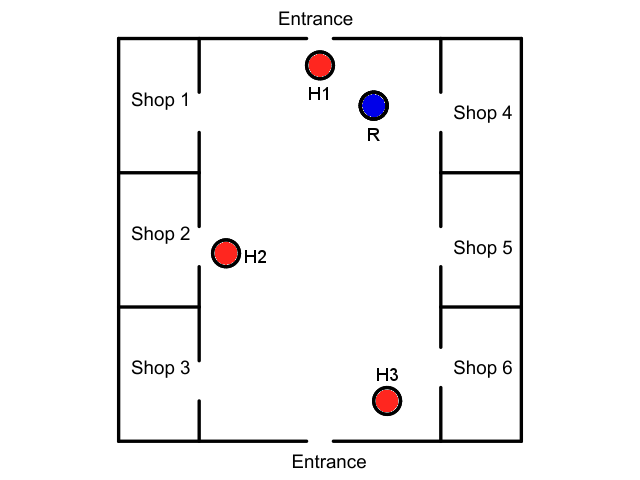
\includegraphics[scale=0.5]{images/mall_situation1.png}
	\caption{A snapshot of the mall, where $R$ is the Robot and $H_i$ a person}
	\label{fig:mall_1}
\end{figure}

\noindent The qualitative information about the people locations indicates that there is a person in front of shop 2, another wandering nearby shop 6 and a third person in front of him. 
\noindent So the set of actions could be represented as \\ 

$A = \{sense\_person, move, bringto, approach\_person, approach\_group, advertise, \\ 
       carry\_bags, wait, ask\_clothes, ask\_food, ask\_object, bye\}$\\ 

\noindent where $X$ could be a generic location or the position of a shop.
\noindent The robot is able to represent knowledge about the environment and try to guess people wishes.
For instance, based on the people locations, he tries to infer from its knowledge if a person is interested in one particular shop or services and could provide an advertisement. 
He maintains an internal database of all the goods for sale, divided by category, so he can better individuate people needs.
If we recap the formula introduced in \ref{sec:approach}, we have that: \\

\centerline{$X = Y \cup Z$}

\noindent where $X$ represents the complete state variables, $Y$ are the environmental state variables while $Z$ are the epistemic state variables. \\

\noindent $Z = \{food, clothes, object, WC, help, none\}$\\
\noindent $Y = \{time, person\_atX, group\_atX, RLocation, foodCategory_i, genericGood_j, \\ clothingStore_k \}$\\

\noindent where $food, clothes, WC, help, none$ represent the person interest in a service, while $FoodCategory_i, GenericGood_j, ClothingStore_k$ represents the specific required goods.\\
Consider person $H2$, that is standing in front of shop 2. \\
Lets assume that 
\begin{itemize}
\item shop 2 and shop 4 are clothes store. The first is a sportive clothes store, while the second is an high fashion store.
\item shop 3 is a WC
\item shop 1 is a market
\item shop 5 and shop 6 are a chinese and an italian restaurant.
\end{itemize}
This situation is summarized in the following figure:
\begin{figure}[H]
	\centering
	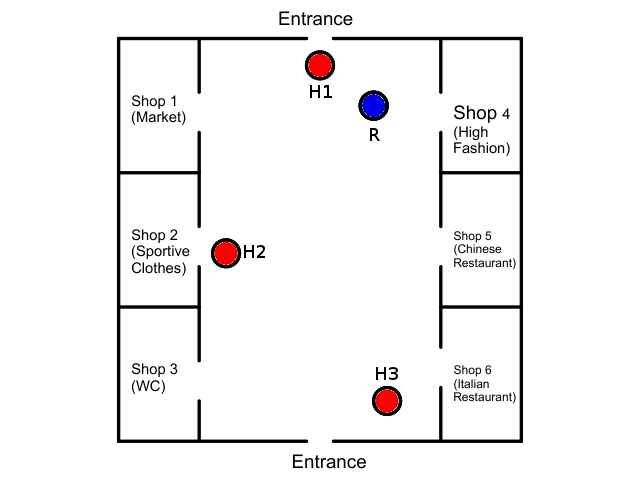
\includegraphics[scale=0.5]{images/mall_situation2.png}
	\caption{}
	\label{fig:mall_2}
\end{figure} 
\noindent We can reasonably think that the person is looking for a specific article inside this shop, or another clothing shop, and that he's not certainly hungry. \\
So a possible plan for $H2$ would be:
\begin{figure}[H]
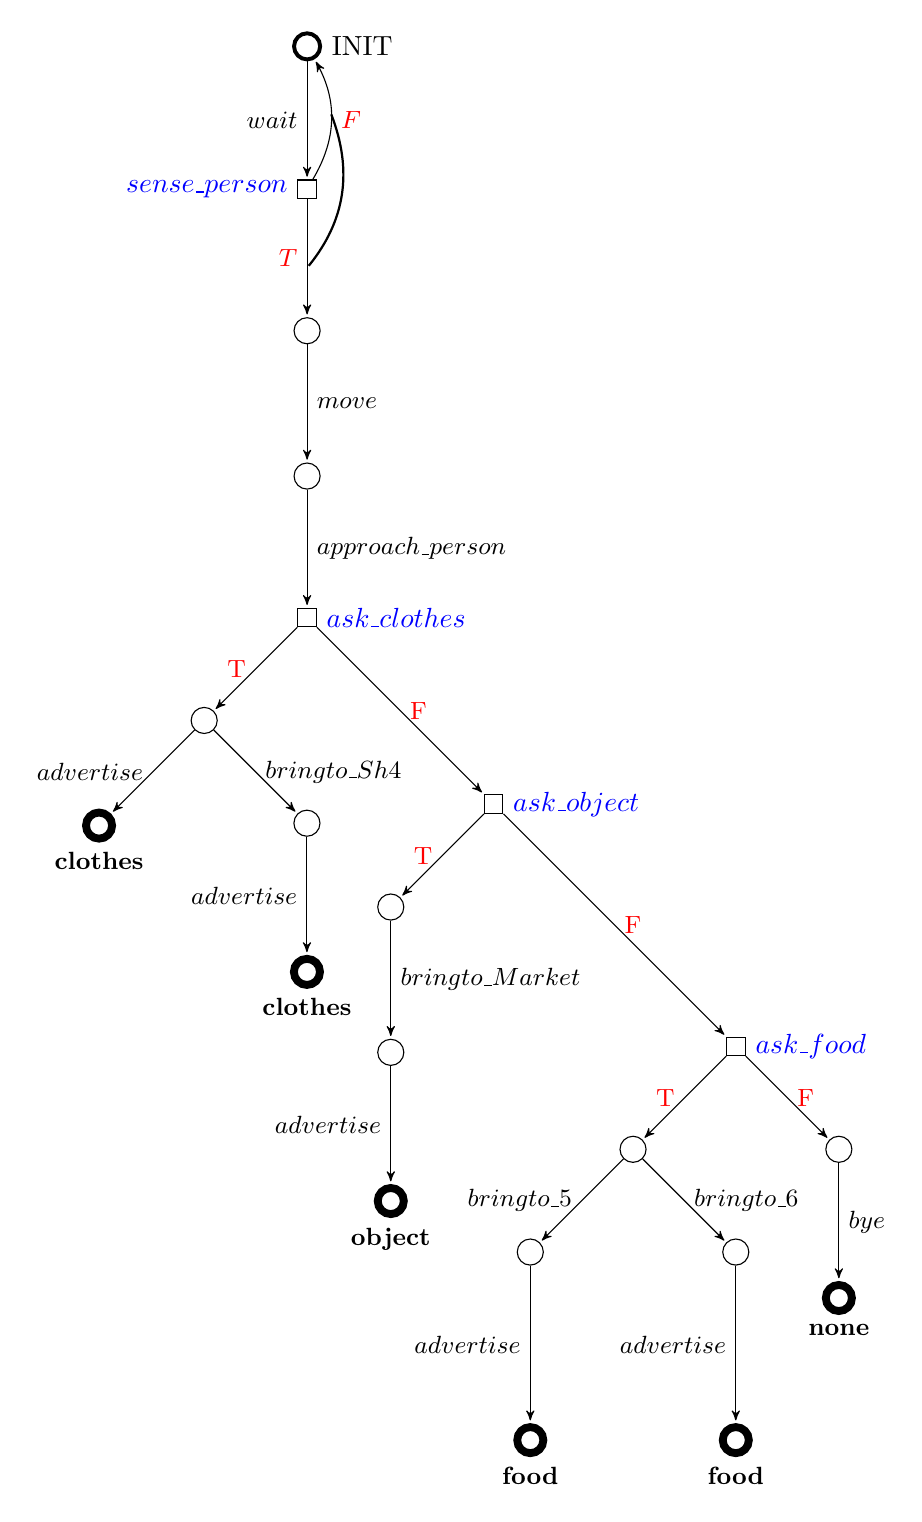
\begin{tikzpicture}[->,>=stealth',shorten >=1pt,auto,node distance=1.5cm,
                    thin,main node/.style={circle,draw,font=\sffamily\Large\bfseries}]

%  \tikzset{every loop/.style={min distance=7mm,in=30,looseness=10}}
%  \node[main node, initial by arrow, initial text={}] [label=right:INIT](S0){\small $S_0$};
%  \node[main node] [below = of S0] (S1){\small $S_1$};
%  \node[main node] [below = of S1] (S2){\small $S_2$};
%  \node[main node] [below left = 2cm of S2] (S3){\small $S_3$};
%  \node[main node] [below = 2cm of S2, right = 2cm of S3] (S4){\small $S_4$};
%  \node[main node] [below = 2cm of S3] (S5){\small $S_5$};
%  \node[main node] [below = 2cm of S4] (S6){\small $S_6$};
%  \node[main node] [below right = of S4] (S7){\small $S_7$};
%  \node[main node] [below = of S7] (S8){\small $S_8$};
%  \node[main node] [below right = 2cm of S7] (S9){\small $S_9$};
%  \node[main node] [below right = 3.5cm of S6] [label=below:GOAL](S10){\small $S_{10}$};
%
%\path (S0) edge [loop above] node {\small $wait$} ();
%\path (S0) edge node {\small $goto\_2$} (S1);
%\path (S1) edge node {\small $approach$} (S2);
%\path (S2) edge node[left] {\small \coloIn this way robot can make assumption about the state of the world, characterize its knowledge, and replan when the outcomes are unexpected.\\r{red} $ask\_clothes$} (S3);
%\path (S2) edge node[right] {\small \color{red} $\neg \,\, ask\_clothes$} (S4);
%\path (S3) edge node[left] {\small $advertise$} (S5);
%\path (S3) edge node[below] {\small $bringto\_X$} (S4);
%\path (S4) edge node[left] {\small $bringto\_WC$} (S6);
%\path (S4) edge node[right] {\small $ask\_food$} (S7);
%\path (S4) edge[bend left=90] node[right] {\small $none$} (S9);
%\path (S5) edge[bend right] node[left] {\small $bye$} (S10);
%\path (S6) edge node[left] {\small $bye$} (S10);
%\path (S7) edge node[right] {\small $bringto\_X$} (S8);
%\path (S8) edge node[right] {\small $bye$} (S10);
%\path (S9) edge node[right] {\small $bye$} (S10);

  \tikzset{every loop/.style={min distance=7mm,in=30,looseness=10}}
  \node[main node, line width=0.5mm][label=right:INIT](init){};
  \node[draw,rectangle] [below = of init](sensep)[label=left:\color{blue}$sense\_person$] {};
  \node[main node] [below = of sensep] (choice1){};
%  \node[draw=none] [left = of choice1] (3dot1) {...};
%  \node[draw=none] [right = of choice1] (3dot2) {...};
  \node[main node] [below = of choice1] (circle1){};
  \node[draw,rectangle] [below = of circle1] [label=right:\color{blue}$ask\_clothes$] (askclot){};
  \node[main node] [below left = of askclot] (choice2){};
  \node[draw,rectangle] [below right = 3cm of askclot] [label=right:\color{blue}$ask\_object$] (askobj){};
  \node[main node, line width=1mm] [below left = of choice2] [label=below:\small\textbf{clothes}](goal1){};
  \node[main node] [below right = of choice2] (circle2){};
  \node[main node, line width=1mm] [below = of circle2] [label=below:\small\textbf{clothes}](goal2){};
  \node[main node] [below left = of askobj] (circle3){};
  \node[draw,rectangle] [below right = 4cm of askobj] [label=right:\color{blue}$ask\_food$] (askfood){};
  \node[main node] [below = of circle3] (circle4){};
  \node[main node, line width=1mm] [below = of circle4][label=below:\small\textbf{object}](goal3){};
  \node[main node] [below left = of askfood] (choice3){};
  \node[main node] [below right = of askfood] (circle5){};
  \node[main node, line width=1mm] [below = of circle5][label=below:\small\textbf{none}](goal4){};
  \node[main node] [below left = of choice3] (circle6){};
  \node[main node] [below right = of choice3] (circle7){};
  \node[main node, line width=1mm] [below = 2.cm of circle6][label=below:\small\textbf{food}](goal5){};
  \node[main node, line width=1mm] [below = 2.cm of circle7][label=below:\small\textbf{food}](goal6){};

\path (init) edge node[left] {\small $wait$} (sensep);
%\path (sensep) edge [bend right] node[right] {\small \color{red} F} (init);
%\path (sensep) edge node[right] {\small \color{red} T} (choice1);
\draw[name path=e1] (sensep) to [bend right] node[right] {\small \color{red} $F$} (init);
\draw[name path=e2] (sensep) to node[left] {\small \color{red} $T$} (choice1);
\path[name path=arc1] (sensep) circle (1);
\draw[name intersections={of=e1 and arc1, by=i1},
      name intersections={of=e2 and arc1, by=i2},
      -,shorten >=1pt,thick]
  (i1) to[bend left] (i2); 
  
%\path (choice1) edge node[above left] {$goto\_Sh6$} (3dot1);
%\path (choice1) edge node[above right] {$goto\_Entr1$} (3dot2);
\path (choice1) edge node[right] {\small $move$} (circle1);
\path (circle1) edge node[right] {\small $approach\_person$} (askclot);
\path (askclot) edge node[left] {\small \color{red} T}(choice2);
\path (askclot) edge node[right] {\small \color{red} F}(askobj);
\path (choice2) edge node[left] {\small $advertise$} (goal1);
\path (choice2) edge node[right] {\small $bringto\_Sh4$} (circle2);
\path (circle2) edge node[left] {\small $advertise$} (goal2);
\path (askobj) edge node[left] {\small \color{red} T}(circle3);
\path (askobj) edge node[right] {\small \color{red} F}(askfood);
\path (circle3) edge node[right] {\small $bringto\_Market$}(circle4);
\path (circle4) edge node[left] {\small $advertise$}(goal3);
\path (askfood) edge node[left] {\small \color{red} T}(choice3);
\path (askfood) edge node[right] {\small \color{red} F}(circle5);
\path (circle5) edge node[right] {\small $bye$}(goal4);
\path (choice3) edge node[left] {\small $bringto\_5$}(circle6);
\path (choice3) edge node[right] {\small $bringto\_6$}(circle7);
\path (circle6) edge node[left] {\small $advertise$} (goal5);
\path (circle7) edge node[left] {\small $advertise$} (goal6);

\end{tikzpicture}
\caption{a plan for H2}
\end{figure}

\noindent Where the squares ($ \square $) represents sensing actions.\\ 
A \textbf{sensing action} is an action that incorporates an observation (a boolean evaluation in this case) and it is used by the robot to characterise its (partial) knowledge of the environment. We assume that a state in which at least one of the $Z$ properties holds is a goal state. \\
\newline
\noindent I will now introduce some formalisms for planning problem representation.\\ 
A more detailed discussion about this formalisms and others will be presented in \ref{sec:formalism}.

\section{Planning: some hints}
Once a problem is characterized, we must define the techniques necessary to solve it.\\
Planning is "\textit{the task of coming up with a sequence of actions that will achieve a goal}" \cite{russell2005ai}.\\
When talking about complex problems, classical search-based planning approaches cease to be useful as any algorithm easily get lost in the possible huge state space.
In this cases, a language for represent the problem represent a better solution.
The convenience of using a formal language is that it guides the planning algorithms through the search of the solution by exploiting the problem logical structure. \\
On other hand, we must deal with some contraindications:
\begin{itemize}
\item \textbf{Uncertainty.} How to deal with uncertainty in action effects and in the state.
\item \textbf{Goal existence.} Does a goal exist? Is it possible to compute it?
\item \textbf{Expressivity vs Complexity.} Can we represent the problem? Is it possible to compute a solution?
\end{itemize} 

\noindent Try to address all this questions is behind the scope of this thesis.\\ 
Instead, I will show how to deal with sensing uncertainty
and how to generate robust plans, that are plans that execute safely with limited or no needs for replanning.\\
\newline
\noindent In chapter \ref{sec:related_works} I will present the context of this work and the state of the art.\\ 
In chapter \ref{sec:plan_repr} I will review some of the formalisms in literature, showing their pros and cons in terms of representation expressivity and computation complexity.\\ 
In chapter \ref{sec:approach} I make some consideration about the analysis done in the precedent chapter and I will introduce the used approach.\\ 
In chapter \ref{sec:foundation} the tools used for the developing of the thesis are presented. In chapter \ref{sec:system} the system is presented, with the architecture and algorithms descriptions.\\ 
Finally, in chapter \ref{sec:use_cases} and \ref{sec:conclusion} some problem examples and considerations about the work are done.
\chapter{Related Works}\label{sec:related_works}
This chapter reviews the state of the art and identifies the field of interest of this work.

\section{Social Robotics}
\textbf{Social Norms}: "\textit{Norms are cultural products (including values, customs, and traditions) which represent individuals' basic knowledge of what others do and think that they should do.}"\footnote{\url{https://en.wikipedia.org/wiki/Norm_(social)}}\\
\newline
\noindent While the previously stated definition of social norms fits very well in an environment populated exclusively by humans, when robots are added to the context it can be very difficult to define what are social norms. In particular, what are the desirable characteristics that a robot must have in order to be defined "social"?\\
\noindent Through recent years we have seen an increasing interest with respect to robotics and artificial intelligence. %TODO aggiungere qualche dato
While the first "intelligent" personal assistants have made their appearance thanks to smartphones diffusion, robots for the major part are still relegated in a factory and seen as fictional characters.
Even in the industrial context, where we can see some examples of human-robot cooperation, the interaction is far from being "social" since the human is seen as an obstacle to avoid and the interaction is programmatic.\\
However, the precedent definition  give us some hints about the fundamental question:\\ 
\noindent\textit{"basic knowledge of what others do and think that they should do."}\\
The importance of developing a robot that is human aware reside in its ability of model human state of mind, especially when we talk about robots that must operate in human environments.\\
We have started to see some examples of robots operating in public environments, and we always come to an end: people are for the most part frightened by robots as they do not know what to expect from it.
Thus, when developing robots for operating beside humans, it is important that the robot has the ability of  drive the interaction, i.e. be an active (not passive) actor. Beside from have an "attractive" design, a robot of this kind must promote different modalities for interaction and maintain at any time a snapshot of person state of mind. The proactivity helps the robot to reduce is uncertainty about the human and ensure, with appropriate behaviours, that the person is always comfortable when in presence of the robot.\\
In general we can state that social robotics norms that are norms of human being imitated/reproduced by the robot in order to encourage collaboration and that are socially acceptable, depending also on the cultural context.\\ 
\subsection{Human Robot Interaction (HRI)}
\textbf{HRI}: \textit{“Understand and shape the interactions between
one or more humans and one or more robots”} (Goodrich\&Schultz 2007)\\
\newline
Human-robot Interaction study the interaction between human and robots. Its a multidisciplinary field, and attracts researcher from robotics, AI, cognitive psychology, and many more.
Its main objective is to develop models for natural and social interaction between humans and robots. 
A central idea in HRI research is that humans expect from a robot to exhibit a human-like behaviour when interacting with them, so they can feel comfortable as when interacting with a person. Is is important to underline that a social robot must interact with non-expert users, that don't know what to expect when dealing with it.\\

\noindent Nowadays the most prominent context in which a social robot could be implied are:
\begin{itemize}
\item Entertainment 
\item Public Environment Assistance (museum, shopping mall, etc.)
\item Shared Tasks (like assisted assembly)
\item Healtcare, elder people assistance, etc.
\end{itemize}

\section{Some Examples}
\subsection{Industrial Cases (No HRI)}
Those are the cases in which robot and human are both aware of the plan and they cooperate deterministically in order to achieve the goal. There is no HRI as the human is seen as another agent in the environment.\\
\textbf{Examples:} \textit{assisted assembly, logistic, space}.

\subsection{Almost Social Cases (HRI Not Mandatory)}
In this cases the interaction between the human and the robot is minimal. The human is a target and the interaction is a secondary objective. No representation of the human state is required.\\
\textbf{Examples:} \textit{patrolling, search \& rescure}.

\subsection{Strictly Social Cases (HRI Mandatory)}
Those cases represents the most significant for this work. In this case the interaction is the principal objective and the robot itself could start the interaction. A representation of the human state is maintained.\\
\textbf{Examples:} \textit{Project COACHES (\url{https://coaches.greyc.fr/}), Amelia the Assistant (\url{http://www.ipsoft.com/amelia/}), assistance task}.


\chapter{Plan Representation}\label{sec:plan_repr}
In this chapter I will discuss about some of the most diffused formalisms and languages for plan representation.
\section{Formalisms}\label{sec:formalism}
\subsection{STRIPS (Classical Planning)}
\noindent STRIPS \cite{fikes1971strips} stand for STanford Research Institute Problem Solver. %\cite{strips}
\\\noindent It is a formal language (and a planner) used to describe deterministic, static, fully observable domains. 
\\\noindent In STRIPS the initial state is assumed to be known with certainty and any action taken at any state has at most one successor (no multiple outcomes). It is not possible to describe indirect effects of actions, as action preconditions/postconditions are expressed simply as conjunction of literals (positive for preconditions).
\\\noindent More formally, a STRIPS instance is a quadruple $<P,O,I,G>$, where:
\begin{itemize}
\item $P$ is a set of conditions (propositional variables).
\item $O$ is a set of operators (actions). Each action is itself a quadruple with four set of conditions specifying which conditions must be true/false for the action to execute and which conditions are made true/false after the execution
\item $I$ is the initial state, specified by a set of conditions that are initially true (all others are false).
\item $G$ specify the goal conditions. This is a pair of two set specifying which conditions must hold true/false in a state in order to be considered a goal.
\end{itemize}
\noindent A plan computed by STRIPS is a linear sequence of actions from initial state to goal state with no branches (i.e. no conditional effects).
\\\noindent This makes STRIPS very fast: the search is done off-line and then the found plan is executed on-line with "eyes closed". 
\\\noindent On other hand it cannot deal with uncertainty in both sensing/knowledge, like unreliable observations, incomplete/incorrect information or multiple possible worlds. Changes to its knowledge must always come from the robot itself and that make it inappropriate for interaction.\\
Not only, when the model became too complex the time to compute a plans grows exponentially, thus making impossible to benefit  of its fastness.
\\\noindent An expanded version of STRIPS is Action Description Language (ADL)\cite{pednault1987formulating}%\cite{adl}, 
which expand STRIPS with some syntactics features:
\begin{itemize}
\item state representation: allows also negative literals.
\item action specification: add conditional effects and logical operators for express them.
\item goal specification: quantified sentences and disjunctions.
\end{itemize}

\subsection{PDDL}\label{pddl}
\noindent PDDL \cite{mcdermott1998pddl} %\cite{pddl} 
is the standard "de facto" for planning domains description. It generalizes both STRIPS\cite{fikes1971strips} %\cite{strips} 
and Action Description Language (ADL \cite{pednault1987formulating}).%\cite{adl}).
\\\noindent It is intended to describe the "physics" of a domain in terms of predicates, possible actions and their effects.
\\\noindent States are represented as a set of predicates with grounded variables and arbitrary function-free first-order logical sentences are allowed to describe goals. 
Action effects are the only source of change for the state of the world and could be universally quantified and conditional. This makes PDDL asymmetric: action preconditions are considerably more expressive than action effects.
\\\noindent The standard version of PDDL divide the planning problem in two parts: domain description and problem description. Domain description contains all the element that are common to every problem of the problem domain while the problem description contains only the elements that are specific for that instance of problem. This two constitute the input for the planner. The output is not specified by PDDL but it is usually a totally/partially ordered plan (a sequence of actions that may be also executed in parallel).
The domain description consist of:
\begin{itemize}
\item \textbf{domain-name}. 
\item \textbf{requirements}. declares to planner which features are used. some examples are strips, universal-preconditions, existential-preconditions, disjunctive-preconditions, adl. When a requirement is not specified, the planner skips over the definition of that domain and won't cope with its syntax.
\item \textbf{object-type hierarchy}.
\item \textbf{constant objects}.
\item \textbf{predicates}.
\item \textbf{actions}. are operators-schemas with parameters, that will be grounded/instantiated during execution. They had parameters (variables to be instantiated), preconditions and effects. Effects could be also conditional. 
\end{itemize}
The problem description is composed by:
\begin{itemize}
\item \textbf{problem-name}.
\item \textbf{domain-name}. to which domain the problem is related.
\item \textbf{objects}. the definition of all possible objects (atoms).
\item \textbf{initial conditions}. conjunction of true/false facts, initial state of the planning environment.
\item \textbf{goal-states}. a logical expression over facts that must be true/false in a goal-state.
\end{itemize}
\noindent I refer to \cite{mcdermott1998pddl}%\cite{pddl} 
for a more formal definition of the syntax.
\noindent Through the years PDDL has received several updates (the last version is PDDL 3.1) and extensions. This enrich PDDL with useful properties that are not present in its standard version, like the possibility of represent uncertainty or probabilistic outcomes for actions.
The most notable are:
\begin{itemize}
\item PPDDL\cite{younes2004ppddl1}%\cite{ppddl} 
is a probabilistic version of PDDL. 
\\\noindent It extends PDDL 2.1 with probabilistic effects, reward fluents, goal rewards and goal-achieved fluents. This allows to realise Markov Decision Process (MDP) planning in a fully observable environment with uncertainty in state-transitions.
\item RDDL\cite{sanner2010relational}%\cite{rddl} 
introduce the concept of partial observability in PDDL. It allows to describe (PO)MDP representing states,actions and observations with variables. Semantically, RDDL represent a Dynamic Bayes Net (DBN) with many intermediate layers and extended with a simple influence diagram utility node reresenting immediate reward.
\item KPDDL\cite{iocchi2003}%\cite{kpddl} 
add to PDDL some constructs to represent the incomplete knowledge of the agent about the environment. It will be discussed in the upcoming sessions.
\end{itemize}

%\subsection{HATP}
%\textit{Characteristics}
%\begin{itemize}
%\item world representetation = collection of entities of type agent/object
%\item Entity = data values + relations with other entities
%\item Initial world state = instantiation of entities with values for attributes
%\item Agent = 1st class entities
%\item Static vs dynamic attributes value (refers to planning); atomic vs set values 
%\item Domain as HTN + variables with controlled binding (SELECT, SELECTORDERED, SELECTONCE)
%\item Partial-ordering allowed for subtasks
%\item Social rules as constraints on parameters/filters, discriminates planes
%\item Geometric reasoning by the means of an interface with geometric planner $\shortrightarrow$ “evaluable predicates”—predicates in HATP preconditions that are evaluated by calling associated external procedures
%\end{itemize}
%
%\textit{Examples}
%\begin{itemize}
%\item Assisted assembly
%\item Dock-worker robot
%\end{itemize}

\subsection{$ALCK_{NF}$}
It is an autoepistemic logic, an extension of ALC with the add of the epistemic operator \textbf{K} and default assumption operator \textbf{A}. It is presented in \cite{donini1997autoepistemic}.%\cite{alck}.
\\\noindent The logic ontology assumes the existence of \textit{concepts} and \textit{roles}. 
\\\noindent A concept represent a class of \textit{individuals} while the roles model the relations between classes.
\\\noindent The interpretation structure of Default logics is a Kripke structure, with labelled nodes and edges.
Each node represents an individual and is labelled with the concept corresponding to the individual while each edge is a role. 
\\\noindent This structures could be interpreted as a dynamic system where the individuals are the states of the system that holds the properties valid in that state (like fluents in situation calculus). Edges represent transactions between system states and are labelled with the action that causes the change in state.
\\\noindent So each node/individual represent an \textit{epistemic state} of the robot so that there is an edge between two nodes if the associated action modifies the source epistemic state in the destination epistemic state.
\\\noindent There are two types of actions: ordinary actions and sensing actions.
\\\noindent  Ordinary actions are deterministic actions with effects that depend on the context they are applied, while the sensing actions do not modify the environment but the knowledge of the agent since they evaluate boolean properties of the environment.
\\\noindent  Thanks to the latter it is possible to explicitly model the effects that this type of actions has on the knowledge and to characterise plans that the agent could actually execute.
\\\noindent It is also possible to specify actions that can run in parallel. Parallel actions in a state can be executed iff each could be executed individually in that state and the effects of the actions are mutually consistent.
\\\noindent For what concerns the Frame problem, the language use default axioms to represent the persistence of properties and frame axioms that express the causal persistence of rules.
\\\noindent Epistemic operators guarantee that the generated plan is actually executable, unlike first-order logic, and sensing actions produces ramifications that could help to reach the goal. This type of plan, with sensing plus ordinary actions, is called conditional plan.

%\subsubsection{Syntax}
%$C \shortrightarrow A$ $|$ $\top$ $|$ $\bot$ $|$ $C_1 \sqcap C_2$ $|$ $C_1 \sqcup C_2$ $|$ $ \neg C$ $|$ 
%$\exists Q.C$ $|$ $ \forall Q.C$ $|$ $\textbf{K}C$ $|$ $\textbf{A}C$ $|$ $Q \shortrightarrow R$ $|$ $R_1 \sqcap ... \sqcap R_n$ $|$ $\textbf{K}R$ $|$ $\textbf{A}R$ 
%
%\noindent where
%\begin{itemize}
%\item $A$ is an atomic concept, there is described only by the name.
%\item $C$ is a complex concept
%\item $R$ is an atomic relation
%\item $Q$ is a complex relation
%\end{itemize}
%
%\noindent An $ALCK_{NF}$ knowledge base is a couple $\Sigma = <T, A>$ where:
%\begin{itemize}
%\item T (TBox
%) is a finite set of inclusion assertions 
%\item A (ABox) is a finite set of assertions of membership C(a) o R(a,b) with a and b individuals names.
%\end{itemize}

\subsection{KPDDL}\label{kpddl_descr}
KPDDL\cite{iocchi2003}%\cite{kpddl} 
is an extension of PDDL based on the logic $ALCK_{NF}$. 
\\\noindent Its aim is to augment the planning domain with the (incomplete) knowledge of the agent about the environment. 
\\\noindent KPDDL introduces several specifications:
\begin{itemize}
\item \textit{sense terms}. effects of actions that helps to disambiguate the true state of the environment.
\item \textit{non-inertial terms}. specifies non-inertial properties. 
\item \textit{strongly-persist terms}. specifies strongly persistence properties.
\item \textit{formula-init term}. is the specification for an incomplete initial state.
\end{itemize}
The fundamental contribute of KPDDL from the semantic viewpoint is the interpretation of a dynamical system through its epistemic state. An epistemic state represents what the agent knows about the world, that could be different from what is true in the world, and the planning is realised by modelling at this meta-level. 
%I refer to \cite{alck} for a complete definition of the introduced constructs.
\\\noindent A planning problem can be specified as:
\begin{center}
$KB \cup \phi (init) \models \pi_{\psi} (init)$
\end{center}
where $KB$ is the set of axioms representing the planning domain, $\phi (init)$ is the assertion representing the initial state and $\pi_{\psi} (init)$ is an $ALCK_{NF}$ assertion that is true in the initial state iff executing the plan agent knows $\psi$. 
\noindent The associated planner produces conditional plans in the form of conditional trees (or direct acyclic graphs), in which the root is the initial states, the leaves are goal states and the branches are different results of sensing. Conditional plans are distinguished in \textit{weak/strong}, whether or not are present leaves that are not goal states and from which a goal state could not be reached. Plans could be also \textit{cyclic}, in which case the termination is not guaranteed.
Formally, a plan is defined as quadruple $P = <G(V,E),I,F_G,F_F>$ where:
\begin{itemize}
\item $G$ is a direct graph, with $V$ nodes and $E$ edges.
\item $I \in V$ is the initial state.
\item $F_G \subseteq V$ is the set of final states in which the goal is achieved.
\item $F_F \subseteq V$ is the set of final states in which the goal is not achieved.
\end{itemize}

\subsection{Answer Set Programming (ASP)}
\noindent Answer set programming (ASP) is a form of declarative programming oriented towards difficult, primarily NP-hard, search problems. \cite{lifschitz2008answer}%\cite{wiasp} 
\footnote{\url{https://en.wikipedia.org/wiki/Answer_set_programming}}
\\\noindent It's declarative in the sense that it describe the problem, not how to solve it.
\\\noindent In particular, a problem instance $I$ is translated into a non-monotonic logic program $P$ and passed to an ASP solver which will search the stable models of $P$. From these, the solution of $I$ is extracted.
\\\noindent ASP programs are composed of Prolog-like rules, but it uses a different computational system. In fact, ASP solvers are based on DPLL algorithm, that in general guarantees the termination (unlike SLDNF resolution in Prolog).
\newline

\noindent A rule has the form:
\begin{verbatim}
<head> :- <body>
\end{verbatim}
where $<head>$ is a disjunction of positive/negative literals, while $<tail>$ is a conjunction of positive/negative literals. 
\\\noindent The symbol :- is dropped if $<body>$ is empty; this are called \textit{facts}. Rules with an empty $<head>$ are called \textit{constraints} and are used to reduce the number of possible solutions (stable models). 
These are useful to express action preconditions like in other formalism (for instance \ref{pddl}).
\\\noindent ASP includes two form of negation: strong ("classical") negation and negations as failure. This allow to represent defaults, useful in order to express the closed world assumption and characterize a solution to the frame problem (inertia of the world: \textit{"everything is presumed to remain in the state in which it is"}).
\newline

\noindent I will now introduce some examples from \cite{lifschitz2008answer}%\cite{wiasp} 
to illustrate ASP properties:
\begin{verbatim}
(1) p :- q.
(2) cross :- not train.
(3) cross :- -train.
\end{verbatim}
\textbf{(1)} is an example of a classic Prolog like rule. It can be interpreted as $q \shortrightarrow p$, that is \textit{"if \textbf{q} hold, than \textbf{p} is in the stable model"}. 
\\\noindent \textbf{(2)} represent an example of negation as failure. This rule represent the knowledge: \textit{"it is safe cross if there are no information about an approaching train"} (not a good idea indeed).
\\\noindent \textbf{(3)} is preferable in this case, since uses the strong negation: \textit{"it is safe cross if it is known that the train is not approaching"}.
\\\noindent If we combine both negations it is possible to express the closed world assumption (\textit{"a predicate does not hold unless there is evidence that he does"}):
\begin{verbatim}
-q(X,Y) :- not q(X,Y), p(X), q(Y).
\end{verbatim}
interpreted as \textit{"\textbf{q} does not hold for a pair of element of \textbf{p} if there are no evidence that it does"}. This allow to include also negative facts about $q$, so to specify the closed world assumption for some predicates and leave the others with the open world assumption.
\\\noindent Finally, it is possible to express time explicitly with constants. This feature is used to define a metric for plans and for express the \textit{"frame default"}:
\begin{verbatim}
p(T+1) :- p(T), not -p(T+1), time(T).
\end{verbatim}
\textit{"\textbf{p} will remain true at time \textbf{T+1} if there is no evidence that becomes false"}.
\noindent ASP programs are often organized in three sections: generate, test and define. The \textit{"generate"} section describes the set of possible solutions while the \textit{"test"} section is used to discard bad solutions. The \textit{"define"} section defines auxiliary predicates used in the constraints. The order of the rules in an ASP program doesn't matter.
\newline

\noindent ASP has been widely used in the service robotics context, both in simulated or real scenarios. Some examples are \cite{erdem2012answer} and \cite{chen2010developing}.%\cite{asp_ex1} and \cite{asp_ex2}.
\\\noindent However, ASP is not well suited for modelling/reasoning about uncertainty in a domain. Incomplete information cannot be handled correctly due to the fact that stable model semantics is restricted to boolean values. Not only, there is no notion of probability and thus all stable models are equally probable. Some extension to ASP with probabilistic information has been proposed, like in \cite{wang2015handling}%\cite{asp+unc1} 
where Markov Logic Networks (MLN) are used. %TODO add some references (ReearchGate requested, Zhang)
\newline

\subsection{Situation Calculus}
Situation Calculus\cite{mccarthy1969some}\cite{reiter1993proving} %\cite{sitcalc1}\cite{sitcalc2} 
is a logic formalism used to represent and reason about dynamical systems. It allows to express qualitative uncertainty about the initial situation of the world and the effects of actions through disjunctive knowledge.
\\\noindent The state is represented as a set of first-order logic formulae. The basic elements are actions, fluents and situations.
\\\noindent A \textit{Situation} is a first order term denoting a state and is characterised by the sequence of actions applied to the initial state in order to reach it. 
\\\noindent \textit{Fluents} are functions or predicates that have as last argument the situation of application and represents properties of a particular situation. Actions may also be parametrized with variables. A fluent differs from a (normal) predicate or function symbol as its value may change from situation to situation.
\\\noindent The binary function symbol $do(\alpha, s) \rightarrow s'$ represent the result of apply action $\alpha$ on a situation $s$, where $s'$ is the resulting situation.
\\\noindent The binary predicate symbol $Poss(.,.)$ represents the possibility of executing an action. For instance, $Poss(\alpha,s)$ is true iff is possible to apply $\alpha$ in situation $s$.

\noindent A Planning Problem in the Situation Calculus is then defined as 
\begin{center}
 $\mathcal{D} \vDash \exists s.Goal(s)$ 
\end{center}
\noindent where $\mathcal{D}$ is a theory of actions, which consists of: 
\begin{itemize}
\item \textbf{Axioms for the Initial Situation}. A formula that represent properties verified in the initial situation $S_0$.
\item \textbf{Unique Name Axioms for the Actions}.
\begin{center}
$do(\alpha_1 , s_1 ) = do(\alpha_2 , s_2 ) \Rightarrow \alpha_1 = \alpha_2 \wedge s_1 = s_2$
\end{center}
Unique name for actions and situations.
\item \textbf{Precondition Axioms}. They codify necessary properties in order to execute actions. 
\item \textbf{Successor State Axioms}. For each fluent establish if is true after the execution of an action. 
Those axioms solve the frame problem as they enforce the persistence of those properties that are not involved or changed by the current actions, describing the causal laws of the domain with an axiom per fluent.
\end{itemize}
\noindent A plan is a sequence of actions that brings the system from the initial situation to a situation that satisfies the condition \textit{Goal(s)}, whenever the formula representing the goal is satisfiable.

%\subsection{$\mathcal{E}^+$}
%The semantics is based on description logic (propositional? more expressive?), that is less expressive than first-order predicate logic but usually decidable wrt it.
%This language allows sensing actions under the assumption that the agent’s sensors are perfect, actions with probabilistic effects, and actions with non-deterministic effects.

\subsection{Markov Decision Process (MDP)}\label{MDP}
\noindent A Markov Decision Process is a stochastic machine state representation of a dynamic system, in which every transition has assigned a probability. This process  is 'Markovian' since Markov property hold, that is the future state depends only on the current action and state and not from the past states.   
\\\noindent The actions to take in every state are specified by a utility function, that guide the agent through the goal and represent the utility of being in a state or take an action. This function specifies a preference over the paths of the graph.
\\\noindent Actions are the only source of change and are assumed to be instantaneous.
\\\noindent In MDP there is no explicit modelling of time. Nor the world dynamics or the reward function depend on absolute time.
\\\noindent A policy $\pi : S \shortrightarrow A$ is a total function that specifies for each state the action to take. The planning problem is then an optimisation problem in which the objective is to find the policy that maximises the expected utility associated with the states and the action.
The goal is represented as a reward and is a deterministic function of the current state.
\\\noindent This it is a quantitative representation, unlike the previously introduced formalisms, in which the uncertainty is represented through probabilistic means (see also \ref{POMDP}).
\newline

\noindent More formally, an MDP is a 5-tuple $\sum = <S, A, P(.,.), R(.,.), \gamma >$ where:
\begin{itemize}
\item $S$ is a finite set of states
\item $A$ is a finite set of actions
\item $P_a(s'|s)$ is the probability that action $ a \in A$ in state $ s \in S$ at time $t$ will lead to state $s' \in S$ at time $t+1$. Notice that $\sum_{s'\in S} P(s,a,s')=1$.
\item $R_a(s'|s)$ is the immediate reward received after the transition from $s$ to $s'$.
\item $\gamma \in [0,1]$ is the discount factor, which weights the importance of the future versus the present rewards.
\end{itemize}

\noindent The probability of a sequence of states $<s_0, s_1, ... , s_n>$ is called history and is defined given a policy as:

\begin{center}
\noindent $P(h | \pi) = \prod\limits_{i \geqslant 0} P_{\pi(s_i)}(s_{i+1}|s_i)$
\end{center}

\noindent The utility function is specified by associating for each $<state, action>$ a cost/reward depending on the value that transition must have for the agent. If we define a cost function as $C : S \times A \shortrightarrow {\rm I\!R}$ and a reward function as $R : S\shortrightarrow {\rm I\!R}$, is it possible to define the utility of execute an action $a$ in the state $s$ as:
\begin{center}
\noindent $V(s|a) = R(s) - C(s,a)$
\end{center}

\noindent Consequently the utility of a policy $\pi$ in a state $s$ is defined as:
\begin{center}
\noindent $V(s|\pi) = R(s) - C(s,\pi(s))$
\end{center}

\noindent and thus for the history:
\begin{center}
\noindent $V(h|\pi) = \sum\limits_{i \geqslant 0} R(s_i) - C(s_i,\pi(s_i))$
\end{center}

\noindent This sum usually doesn't converge and we need a discount factor $\gamma$ in order to reduce the effect of costs/rewards distant from the actual state.
\\\noindent Introducing $\gamma$, we can rewrite the utility of the history as:
\begin{center}
\noindent $V(h|\pi) = \sum\limits_{i \geqslant 0} \gamma_i (R(s_i) - C(s_i,\pi(s_i)))$
\end{center}

\noindent with $0 < \gamma < 1$. With a value of $\gamma$ near 1 we promote immediate rewards over futures, while with $\gamma \cong 0$ the vice versa.
\noindent From the history utility is possible to calculate the expected value of a policy utility by considering all the history that the policy induce.
Given $H$ as the et of all possible history induced by $\pi$, this expected value is:
\begin{center}
\noindent $E(\pi) = \sum_{h \in H} P(h|\pi)V(h|\pi)$
\end{center}

\noindent a policy $\pi^*$ is said to be optimal for a stochastic system $\Upsigma$ if:
\begin{center}
\noindent $E(\pi^*) \geqslant E(\pi) \,\,\,\, \forall\pi$ 
\end{center}

\noindent where $\pi$ is an admissible policy for $\Upsigma$.
A solution to an MDP is then a policy that, once found, is applied in any state in a deterministic fashion.
\newline

\subsection{Partially Observable MDP (POMDP)}\label{POMDP}
In many cases, the assumption of complete observability for the state is too strict so Partially Observable MDP was introduced.
\\\noindent In this case, a set of observations is defined that characterise the observable part of the stochastic system $\Upsigma$. 
%This subset of the states is represented by probability distributions over the states themselves, introducing a representation of the uncertainty.

\noindent A POMDP is a stochastic system $\Upsigma = <S,A,P(.,.)>$ as defined in \ref{MDP}, with the addition a finite set of observations $O$ with probability $P_a(o|s)$ for all $a \in A, s \in S, o \in O$. $P_a(o|s)$ represent the probability of observe $o$ in the state $s$ after the execution of $a$. This is defined for every state/action and the condition  $\sum\limits_{o \in O} P(o|s)=1$ hold.

\noindent More than one observations could correspond to one state (i.e. $P_a(o|s) = P_a(o|s')$) and thus is not possible to obtain the actual state from the observations.
Analogously the same state could correspond to different observations depending on the action executed, that is 
$P_a'(o|s) = P_a(o|s)$. 
Thus observations depend both on the state and on the action. For instance, a sensing action does not modify the state of the system but could lead to a different observation.

\noindent Probability distributions over the states are called \textit{belief states}. Let be $b$ one belief state and $B$ the set of all belief states. Then $b(s)$ denotes the probability for the system to be in state $s$.

\noindent In order for $b(s)$ to be a probability distributions both $0 \leqslant b(s) \leqslant 1$ and $\sum\limits_{s \in S} b(s)=1 \,\,\, \forall b \in B$ must hold.
Given an action $a$ and a belief state $b$, the next belief state deriving from apply $a$ in $b$ is:
\begin{center}
\noindent $b_a(s) = \sum\limits_{s' \in S} P_a(s|s')b(s')$ 
\end{center}

\noindent Similarly we could compute the probability of observe $o$ given the action $a$:
\begin{center}
\noindent $b_a(o) = \sum\limits_{s \in S} P_a(o|s)b(s)$ 
\end{center}

\noindent At last, we can compute the probability of being in $s$ after executing $a$ and observing $o$:
\begin{center}
\noindent $b_{a,o}(s) = \frac{P_a(o|s)b_s(s)}{b_a(o)}$ 
\end{center}

\noindent Planning in POMDPs is formulated as an optimization problem over the belief space to determine the optimal policy $\pi^* : B \shortrightarrow A$ with respect to an utility function defined as in \ref{MDP}. In fact we can see at a POMDP as a continuous MDP where the continuous space is the belief space.
\\\noindent The expected value for the utility of a belief state $b$ is defined as:
\begin{center}
\noindent $E(b) = \min\limits_{a \in A} C(b,a) + \gamma \sum\limits_{o \in O}b_a(o)E(b_{a,o})$ 
\end{center}
\noindent where:
\begin{center}
\noindent $C(b,a) = \sum\limits_{s \in S}C(s,a)b(s)$ 
\end{center}

\section{Analysis of Formalisms}\label{sec:analysis}
The introduced formalisms and models show the essential bond between expressiveness and computational complexity. The planning problem in classic logic is decidable but the complexity varies from constant to EXPTIME depending on which characteristics are added to the language. 
\newline

\noindent For instance, STRIPS is the less expressive of the presented formalisms, still deciding whether a plan exists is PSPACE-complete \cite{bylander1994computational}.%\cite{strips_comp}. 
Many restrictions can be enforced in order to make this problem decidable in polynomial time, like restricting the type of formulas or the number of pre-postconditions. 
\newline

\noindent $ALCK_{NF}$ is an example of decidable formalism with a good expressiveness, since it allows to express the agent epistemic state explicitly. However the planning in its most general case falls in PSPACE complexity, thus intractable for an online approach. In this and similar cases, partial planning and restricted version of the formalism are used in order to solve the complexity problem.
\newline

\noindent In KPDDL is it possible to express incomplete information through epistemic states and define sensing actions that help to disambiguate the states. In practice, however, it was seen that even a small variation in the number of states makes the problem intractable, proving that the class of complexity is at least PSPACE (instance checking/reasoning in $ALCK_{NF}$ is PSPACE-complete \cite{donini1997autoepistemic}.%\cite{alck}). 
\newline

\noindent Talking about POMDPs models, they are often computationally intractable to solve exactly and thus it is necessary to introduce methods to approximate solutions. Some examples are \cite{roy2005finding}%\cite{belief_compression} 
and \cite{brafman2014contingent},%\cite{belief_particle}, 
where particle filters and PCA are respectively used to represent the belief state compactly or exploit its properties.
\newline

\noindent Planning with partial observability is the most difficult planning task as it falls in EXPSPACE-complete class of complexity \cite{rintanen2004complexity}. The difficulty resides in the plan verification since the state space, in this case, is doubly exponentially bigger in the size of the problem instance with respect to classical planning case.
The discussion of good heuristics and search algorithms that try to exploit the structure of such problems is not the purpose of this thesis.
We will focus instead on the representation of the state space, relying on state of the art planners present in literature.

%\newpage
%\subsection{Bechmarks Experiments} \label{sec:benchmarks}
%In the following I will list some benchmarks domain problems. \\ 
%Most are common to the planning community and are taken from international competitions like IPC (International Planning Competition). \\
%It is somehow difficult to derive a complete and unbiased problem instance, as every new language/planner usually comes with its testing domains and this are most of the time uncommon.  
% 
%
%\subsubsection{STRIPS/PDDL}
%\begin{itemize}
%\item Block World
%\item Classical Planning Domains (IPC problems collection)
%\end{itemize}
%
%\subsection{HATP}
%\begin{itemize}
%\item Assisted assembly
%\item Dock-worker robot
%\end{itemize}
%
%\subsection{ASP}
%\begin{itemize}
%\item Evolutionary studies
%\item Natural language processing: Dependency parsing, linguistics, taxonomy, inferring Phylogenetic Trees
%\item Graphs: graph colouring, Large clique, Hamiltonian cycle
%\item Decision Support for the Space Shuttle
%\item Automated Product Configuration
%\item Coaches
%\end{itemize}
%
%\subsection{MDP}
%\begin{itemize}
%\item SPUDD: grid world, coaches
%\item Often in combination with other formalisms, any task with probabilistic outcomes (perception/state)
%\end{itemize}
%\subsection{POMDP}
%\begin{itemize}
%\item grid world with probabilistic outcomes (faulty navigation)
%\end{itemize}
%
%\subsection{Various}
%\subsubsection{Waitress Robot}
%A mobile Robot with wheels and two arms has to serve clients in a restaurant environment. One of the arms is a tray where he can put 3 food/cocktail at maximum. He has also sensors to perceive the environment.
%He transports the goods from the kitchen to the clients, taking ordinations from them and welcoming incoming persons. After he has received a client, he must bring him to the table and take the ordination. He could take multiple ordinations, but he must reply sooner to the cook when a food is ready. Every food has its maximum delivery time before it gets cold (discrete values from 1 to 3 minutes). Cocktails have no delivery time.
%People could also recall the attention of the robot by the means of a button on the table so that they can order more foods/drinks. So the task priority is:
%\begin{enumerate}
%\item deliver goods
%\item welcome person and take ordination
%\item take random ordinations
%\end{enumerate}
%
%\noindent  An object on the tray could fall down with a probability 0.4, so every time the robot deliver goods he must check if the object is effectively on the tray. If not he must notify the kitchen. The kitchen and the main room are connected via a door that could be both closed or open with equal probability and the robot must check its condition each item. Due to the ambient condition, he could also fail any perceive action with probability 0.2. If the door is closed and the robot doesn't perceive it, all the goods will fall certainly (if is there are any). The goal is to minimize the waiting time both for the clients and the cook given the previous priority list.

%\subsubsection{Assisted Assembly}
%This example is inspired by the one presented in \cite{alami2014human} \\ %\cite{alami}.\\
%In assisted assembly task a robot must bring tools to a worker and helps him with a welding procedure. The robot is a humanoid, thus with two arms and two legs, and has a perception system. The environment contains cavities that only the robot could pass in order to reach the worker or move a particular tool from one room to another. The worker is standing in front of its working table. 
%The worker access is working station through a manhole that remains open all the time, costituting a threat for the robot. If the robot cross all the the worker room he could fall down in the hole with probability 0.6.
%Tools are placed randomly in other rooms and the robot knows exactly where they are through a system of external cameras. When the worker requires a tool, he must bring him as soon as a possible minimizing the traveled rooms. There are 8 rooms and they are all accessible through the cavities. Cavities requires that the robot assumes particular configurations in order to pass through. Each configuration of the robot could be evaluated by a predicate that tells in constant time if the robot will pass or not, but this valid configurations changes according to the number and the type of tools transported. The robot has N degrees of freedom. For the assembly part of the task, the input of the problem is the kinematic model of the robot with its initial configuration, the representation of the environment and the tools required by the worker. The output is all the configurations that the robot must assumes in order to full fill the requirements, that are brings all the tools and minimize worker waiting time. \\
%
%\noindent In the assisted welding the robot stays in the same room of the worker and, since he has better understanding of spatial geometry, he must indicate to the worker the exact trajectory of the welding.
%In this case the input of the problem are the initial configurations of both the robot and the worker, and the output must be a sequence of configurations that minimizes the change in stance of the worker according to some comfort measurement parameter that evaluates worker configurations.

%\subsubsection{COACHES}
%This examples are taken from \cite{iocchi2016practical}%\cite{coaches}.
%\newline
%\\\noindent \textbf{Basic Service Robot}\\
%A robot is able to execute two activities A and B upon request of the user, but the user does not know about these robot abilities. The robot is normally in a waiting state. Whenever a user is detected in front of the robot (for example, with a simple face detector procedure), the robot can decide whether to start an interaction (for example, through a spoken dialogue) and, if so, it describes the activities that it can do A and B. The user can now select one of them or answer that s/he is not interested (for example by selecting an option on a user interface or by a speech command). If a goal is selected, the robot executes a task for achieving it. Each goal can be achieved with two alternatives tasks \textit{TaskA1} and \textit{TaskA2} for \textit{A} and \textit{TaskB1} and \textit{TaskB2} for \textit{B}. After the execution of the task, the robot comes back to the wait state, waiting for a next user. During the execution, the following inconveniences may occur: the user does not complete the interaction (for example, s/he does not answer the robot question), any task may fail for reasons not modeled in the task description, and any task may be aborted according to some external command or condition.
%\newline
%\\\noindent \textbf{Service Robot assisting customers of a shop-ping mall}\\
%A robot operates in the corridor of a shopping mall including several shops. Each shop-keeper can define a set of advertisements that the robot is asked to communicate to customers of the mall and each advertisement has an associated reward for the shopping mall. The robot can execute the following actions in the environment: move to any location (i.e., in front of any shop), approach a specific person or a group of people, perform advertisement actions, perform other assistive actions upon request, bring a person to any location in the mall. The problem we want to solve is the following: given the current position of the robot, the information about shops and advertisements and an initial probability distribution of the presence of people in the shopping mall (for example, provided by an external system of video-cameras), plan and execute the behavior that maximizes the global actual reward, also recovering from possible failures due to unpredicted or erroneous interactions with people.

\chapter{Conditional Planning and Execution}\label{sec:approach}
In this chapter I will explain the reasons behind this work.\\
\newline
\noindent As we have seen in the previous chapter, different planning formalisms try to capture different aspects of real-world problems. By the way they model and abstract the world, they also produce different solution concepts.\\
Is not always obvious in advance which formalism is the best for a specific problem. Less expressive formalism are often preferred due to the fact that are less expensive in terms of computational power.\\
For instance if we consider decidable logic formalisms, $ALCK_{NF}$ is one of the more expressive and yet the planning in general it's included in PSPACE, so too complex to run on a real robot in realtime.\\ 
Classical Planning models only deterministic actions, and the planner is often embedded in a controlled execution loop that replan on unexpected outcomes. In fully-observable and non-deterministic planners, actions are assumed to be non-deterministic but there is no uncertainty about the perception. They produce strategies that are guaranteed to reach the goal. \\
If we expand the domain and consider also probabilistic planners, they introduce also outcome probabilities. Their aim is to maximise a cumulative reward. They are also the most expensive and often intractable at representation and/or execution level. \\
Rule-bases are not manageable when they become larger. This rules are created by experts that express their knowledge through the rules and it is difficult to find all the inconsistencies and the side-effects when new rules are inserted.\\


\noindent This brief analysis shows that there is a compromise between expressivity and computational complexity. 
Epistemic logics could helps us to represent real world uncertainties.\\
In this case the states of the planning problem are called belief states, since they represent the uncertainty of the agent about the world.
The problem with this representation is that the belief space is computationally exponentially bigger than classical state space. A good representation is thus needed.\\
A solution is to maintain only a small group of states that represents a compact description of the epistemic knowledge of the robot.\\
So if we denote as $Z$ the states that represents the epistemic knowledge and with $Y$ the generic states, we have that:
\begin{center}
$|Y|$ + $|2^Z| \ll |2^X|$ and $X = Y \cup Z$
\end{center}

\noindent The next step is to identify a group of formalisms from the ones described in \ref{sec:formalism} that allow us to represent explicitly the epistemic state.\\
In our case, a language must supply the syntactic constructs to define sensing actions with which we can represent conditional plans.
We can identify a bunch of properties that helps make this choice, as we can see from the following table:
\begin{figure}[H]
	\centering
	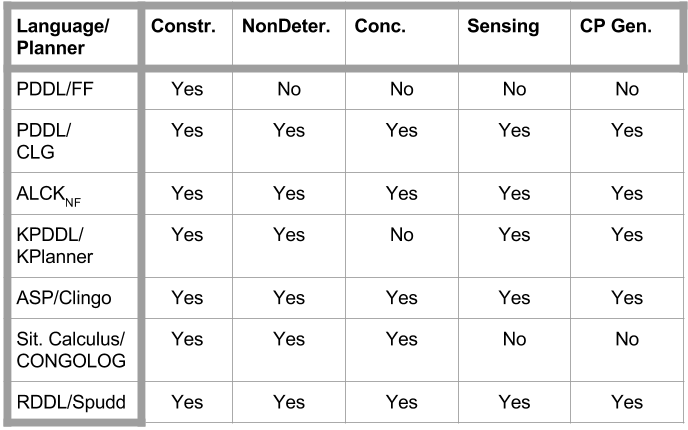
\includegraphics[scale=0.4,trim=30mm 0mm 0mm 0mm]{images/formalisms.png}
	\caption{a comparison betweem different formalisms/planner.}
	\label{fig:formalisms}
\end{figure}
Where the properties showed are:
\begin{itemize}
\item \textbf{Constr.}: the capability of define domain constraints.
\item \textbf{NonDeter.}: the capability of define non-deterministic actions.
\item \textbf{Conc.}: the capability of define concurrent actions.
\item \textbf{Sensing}: the capability of define sensing actions.
\item \textbf{CP Gen.}: the capability (of the planner) to generate conditional plans.
\end{itemize}
\noindent As we can see, PDDL (ROSPlan version), KPDDL, ASP and RDDL seems to fit our prerequisites. For this work we decide to consider the two version of PDDL (standard and ROSPlan) plus KPDDL. We will motivate this choice in the upcoming chapters.\\
\noindent Once we have identified the languages that matches our prerequisites, we select them to represent and  solve a test domains. The last step is to translate the computed plan into a conditional plan as we will discuss later.\\
%\noindent The next step is to identify the a group of formalisms from the ones described in \ref{sec:formalism} that allow us to represent the epistemic state. \\
%This is done in the following table: 
%\begin{itemize}
%\item Huge state space
%\item Decomposable
%\item Hard Synchronization
%\item Non-deterministic observation
%\item Non-deterministic outcomes
%\end{itemize}
\noindent Summarizing, our aim is to define an architecture capable of translate different formalisms into a conditional plan that will represent a PNP, in order to satisfy some tasks requirements, while finding the best trade-off between complexity and expressivity. \\

\chapter{Foundation Tools}\label{sec:foundation}
In the following I will illustrate the tools used for the development of this thesis.

\section{Petri Net Plan}\label{petrinet}
We need a language that can represent non-instantaneous and conditional actions. \\
Petri Net Plans (PNP)\cite{ziparo2006petri}%\cite{pnp}
\cite{ziparo2008pnp}%\cite{pnp2} 
is a formalism for represent complex plans using an high-level description.
It is inspired by languages for reasoning about actions, like the ones presented in \ref{sec:formalism}, but it is more expressive and offer all the operators needed for representing conditional plans, concurrent actions and multi-agent plans.
They also offer non-deterministic choice operator for representing non-deterministic choice action, useful in learning algorithms. \\
The execution of a PNP is very efficient, and allow the design of real-time and active behaviours.
Some examples of PNPs applications are \cite{bastianelli2013line}\cite{palamara2008robotic}\cite{farinelli2006assignment}.
%\cite{pnp_app}\cite{pnp_app2}\cite{pnp_app3}.	

\subsection{Formal Definition}
A PetriNet Plan is a PetriNet augmented with a set of goal markings $G$.
More formally, it is a tuple $<P,T,F,W,M_0,G>$ where:
\begin{itemize}
\item P = \{$p_0, ... ,p_n$\} is a finite set of places.
\item T = \{$t_0, ... ,t_n$\} is a finite set of transitions.
\item $F \subseteq (P \times T) \cup (T \times P)$ is a set of edges.
\item $W: F \Rightarrow {1,2,3,...}$ is a weighting function.
\item $M_0: P \Rightarrow {0,1,2,...}$ is the initial marking.
\item $P \cup T \neq  0 $ and $P \cap T = 0$
\end{itemize} 

\noindent Petri Nets represent the structure of a system as a directed, weighted and bipartite graph with two type of nodes: places and transitions. With this tools we can model complex systems in terms of their internal state and its changes.
\begin{figure}[H]
	\centering
	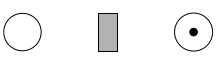
\includegraphics[scale=0.6]{images/place_trans_token.png}
	\caption{(1) a place. (2) a transition. (3) a place with one token.}
\end{figure}
\noindent Places represent the execution phases of an action, while transitions represent events.
In particular each action is represented by three states: initial, execution and final state. Between them there are action starting transition, action terminating transition and there might be some action interrupts and/or control transitions. \\
The evolution of the Petri Net is described by the firing rule: a transition is enabled when the number of tokens for its initial places is equal at least to the number of tokens of the edge weight.
When the transition fires, a number of tokens equal to the weight of the input edges is removed from the initial places and a number of tokens equal to the output edges is added to output nodes.
Petri Net Plans are defined in terms of actions and operators. There are three types of actions:
\begin{enumerate}
\item \textbf{no-action}. is a PNP with one place and no transition.
\item \textbf{ordinary-action}. is a PNP with three places and two transitions, as described before.
\begin{figure}[H]
	\centering
	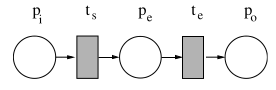
\includegraphics[scale=0.5]{images/ordinary_action.png}
	\caption{an ordinary action.}
\end{figure}
\item \textbf{sensing-action}. this are used when the action involve a property to evaluate at run time, and places/transitions are defined accordingly.
\begin{figure}[H]
	\centering
	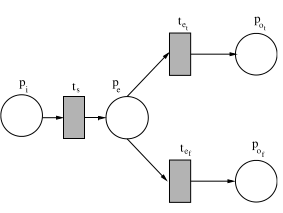
\includegraphics[scale=0.5]{images/sensing_action.png}
	\caption{a sensing action.}
\end{figure}
\end{enumerate}

\noindent Actions could be combined in order to achieve complex behaviours. These are called operators.
\begin{itemize}
\item \textbf{sequence}. allows the execution of two actions in sequence.
\begin{figure}[H]
	\centering
	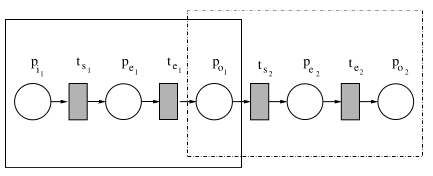
\includegraphics[scale=0.5]{images/sequence.png}
	\caption{sequence operator.}
\end{figure}
\item \textbf{conditional}. combining sensing action with ordinary actions is possible to obtain conditional structure.
\begin{figure}[H]
	\centering
	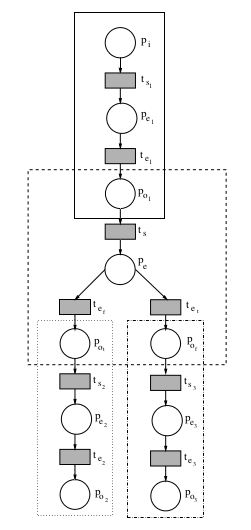
\includegraphics[scale=0.5]{images/conditional.png}
	\caption{conditional operator.}
\end{figure}
\item \textbf{interrupt}. allows to interrupt the execution of an action, if some condition is met, and to continue the execution on a new branch.
\item \textbf{loop}. using an interrupt, is possible to define action that iterates until a condition is true.
\begin{figure}[H]
	\centering
	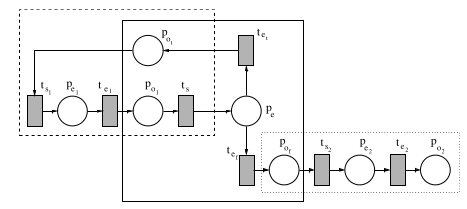
\includegraphics[scale=0.5]{images/loop.png}
	\caption{loop operator.}
\end{figure}
\item \textbf{fork/join}. allows concurrency. fork generates multiple threads starting from one, while join allow the synchronization of multiple threads into one.
\begin{figure}[H]
	\centering
	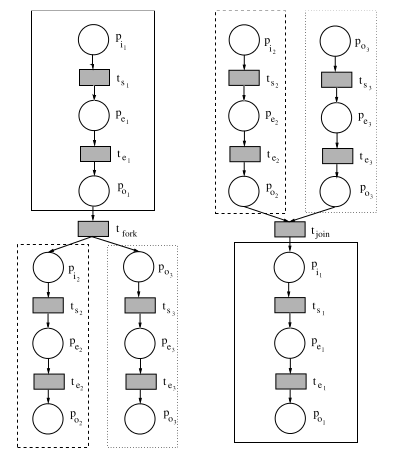
\includegraphics[scale=0.5]{images/fork_join.png}
	\caption{(left) fork operator. (right) join operator.}
\end{figure}
\end{itemize}

\noindent In the following page there is an example of a complete PNP, with an interrupt defined during the action \textit{followperson}:
\newline
\begin{figure}[H]
	\centering
	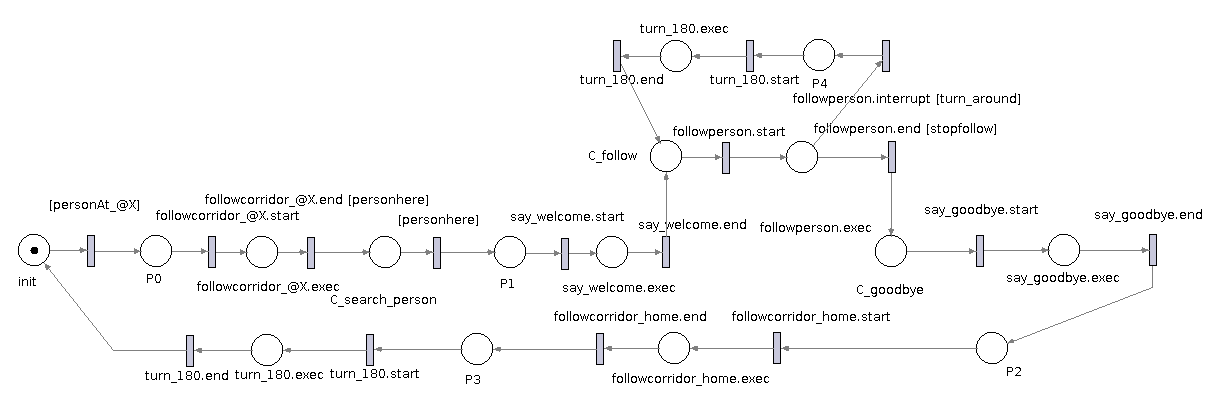
\includegraphics[scale=0.4,  trim=20mm 10mm 10mm 10mm]{images/go_and_follow_person.png} %angle=270,
\end{figure}

\section{PNPgen}
PNPgen\footnote{\url{https://sites.google.com/a/dis.uniroma1.it/petri-net-plans/pnp-generation}}\cite{carlucci2015explicit}%\cite{pnp_gen} 
is a library included the Petri Net Plans distribution responsible for the automatic generation of PNPs from a formal definition provided.\\
This is usually used in conjunction with a planner, which output is interpreted and executed as a PNP.\\
The main advantages of this approach are two:
\begin{enumerate}
\item The produced plan can be executed and monitored through the PNP execution engine and easily integrated into ROS thanks to the PNP-ROS bridge.
\item Once produced,the PNP can be extended of modified to deal with unexpected outcomes that may arise during the execution of an action and not considered in the domain, either manually or automatically as we will discuss later.
\end{enumerate} 

\noindent Furthermore, when used in combination with a formal language we can describe and generate plans that are otherwise too complex to be constructed manually (using a visual editor, i.e. Jarp).
Some examples of PNPgen input are enlisted in the following. Conditional plans generation is discussed in \ref{sec:generator} and \ref{sec:use_cases}.
\subsection{Linear Plans}
PNPgen is able to generate linear plans from a file that describes a sequence of actions to execute, separated by semicolons. An example of a valid file is:
\begin{center}
\texttt{goto\_printer; say\_hello; goto\_home}
\end{center}
saved in a ".plan" file. When this file is given as input to PNPgen, the following PNP is generated:
\begin{figure}[H]
	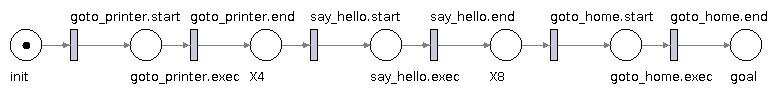
\includegraphics[scale=0.6]{images/linear_plan.png}
	\caption{a simple linear plan.}
\end{figure}

\subsection{Policy}
Another valid format for PNP plans generation is represented by policies. Policies are transition graphs with non-deterministic and sensing actions, that enhance the robustness of the described plan.
For instance, consider the following valid file describing a policy:

\noindent\texttt{Init: S0\\
Final: S3\\
S0 : goto\_printer -> { [personhere] S1, [not personhere] S2 } \\
S1 : say\_hello -> { [] S2 } \\
S2 : goto\_home -> { [] S3 }}\\

\noindent This generates the following PNP:
\begin{figure}[H]
	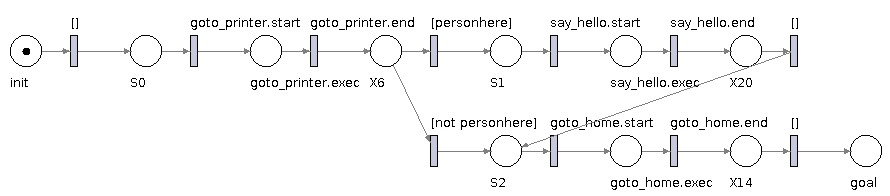
\includegraphics[scale=0.5]{images/SimplePolicy.png}
	\caption{a PNP generated from a a policy.}
\end{figure}
\noindent Where we can see that the property "\textit{personhere}" is evaluated at execution time in state 1, enhancing the plan robustness.

\subsection{Execution Rules}
In both the introduced cases, is it possible to specify an execution rules file as a support to the PNP generation mechanism. \\
This is a file that enlists a series of rules describing possible exogenous events that may occur during the execution of an action. These rules introduce interrupt in the specified action. \\
\newline
For instance, consider the following execution rule:
\begin{center}
\texttt{*if* (and personhere (not closetotarget)) *during* goto *do* say\_MoveAway; waitfor\_freespace; restart\_action}
\end{center}
this led to the introduction of a branch in the following PNP:
\begin{figure}[H]
	\centering
	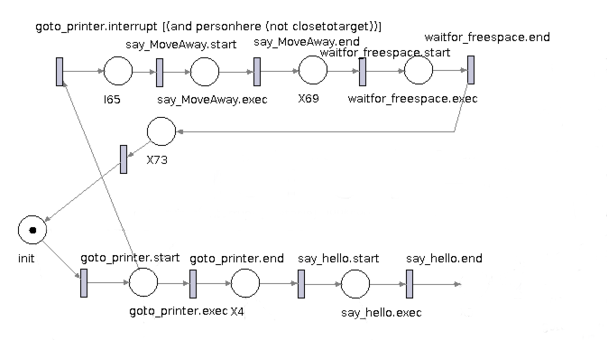
\includegraphics[scale=0.6]{images/er_example.png}
	\caption{an execution rule example.}
\end{figure}
\noindent The syntax of an execution rule is:
\begin{center}
\textbf{if} ($\phi$) \textbf{during} \textit{a} \textbf{do} \{$\sigma; \rho$\}
\end{center}
Where $\phi$ is a boolean expression over some properties, \textit{a} is an action, $\sigma$ is a (possible empty) program (i.e. a sequence of actions, another PNP, etc.), and $\rho$ is a statement that specifies how to continue the execution of the plan (like \textit{restart action, skip action, restart plan, fail plan}). Execution rules are described in \cite{iocchi2016practical},%\cite{coaches}, 
where also a third method to generate PNPs from progressive reasoning unit (PRU) is discussed.

\newpage
\section{Robot Operating System (ROS)}
"Robot Operating System (ROS) is a collection of software frameworks for robot software development, providing operating system-like functionality on a heterogeneous computer cluster. ROS provides standard operating system services such as hardware abstraction, low-level device control, implementation of commonly used functionality, message-passing between processes, and package management. Running sets of ROS-based processes are represented in a graph architecture where processing takes place in nodes that may receive, post and multiplex sensor, control, state, planning, actuator and other messages." \footnote{\url{https://en.wikipedia.org/wiki/Robot_Operating_System}}
\newline

\noindent ROS was originally developed at Stanford Artificial Intelligence Laboratory in support of the Stanford AI Robot STAIR (STanford AI Robot) project. From 2008 to 2013 the development take place at Willow Garage, a robotics research institute. Finally, from 2013, ROS become part of the Open Source Robotics Foundation.\\
During all this time, ROS has growth in importance and diffusion. \\
In fact, before ROS advent, each laboratory or research group had to write down from scratch specific code for his platform and for every task, even the more mundane. This not only is a time expensive task but restrains the diffusion of new algorithms and ideas.
With the layer of abstraction offered by ROS, it is possible to write nodes for common tasks and specific hardware that are reusable and so more easy to diffuse. For instance, ROS offers packages for perception, object identification, segmentation and recognition, face recognition, planning, grasping, localization, mapping and much more. The main limitation of ROS resides in its latency since is built on top of Linux and is not a real-time OS. This led to the born of ROS 2.0, which support real-time operations, and RT-ROS, which is natively real-time. %TODO talk about STAGE and actionlib module

\section{PNPros}
PNPros serves as bridge between ROS and PNP.\\
It allows the execution of PNP under ROS using the \textbf{actionlib} module.\\ 
Like for standard actionlib nodes, it implements the client/server protocol through the definition of an Action Server, called \textbf{PNPActionServer}, and an Action Client, \textbf{PNPActionClient}.\\ 
They communicate through the use of \textbf{PNPAction} messages.\\ 
Furthermore, PNPros defines a service, \textbf{PNPConditionEval}, that is invoked to evaluate conditions at runtime.\\
A sketch of the PNPros architecture is depicted below:
\begin{figure}[H]
	\centering
	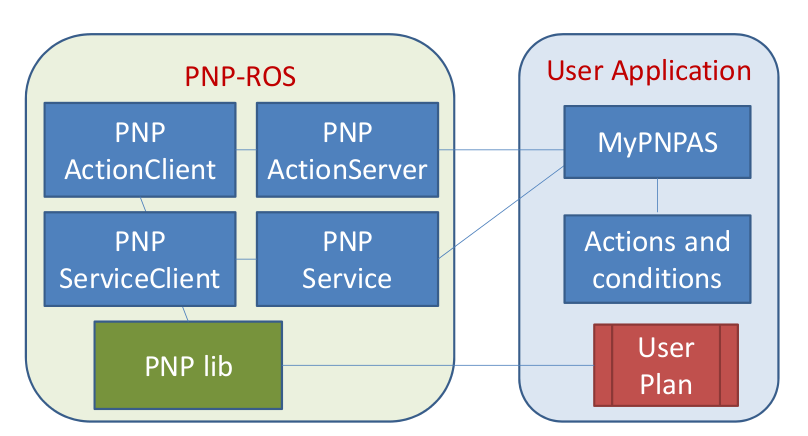
\includegraphics[scale=0.4]{images/pnpros.png}
	\caption{the PNPros architecture.}
\end{figure}
\noindent As we can see, the user must provide its own implementation of the server, actions and the conditions to be evaluated. 
PNPros actively listens a topic for plans to execute; as soon a plan is sent, it starts the execution and monitoring of the PNP. When needed, it will invoke PNPActionServer to evaluate a condition or execute an action. The actions provide the actual low-level implementation (typically in C++).\\
Finally, PNP plans can be written and monitored using Jarp, a graphical tool interface written in Java.

\section{ROSPlan}\label{sec:rosplan}
ROSPlan\cite{cashmore2015rosplan}\footnote{\url{http://kcl-planning.github.io/ROSPlan/}} is a framework that provides a general method for task planning in ROS.
It encapsulates both planning and dispatch and, thanks to its modular design, it is easy to modify to test new approaches to plan representation, plan execution, etc.\\
The main modules are the \textbf{Knowledge Base}, that stores PDDL models, and the \textbf{Planning System}, that is the interface to the planner. The Planning System itself is composed of three modules, which are replaceable: problem generation, planning, and plan dispatch. 
\begin{figure}[H]
	\centering
	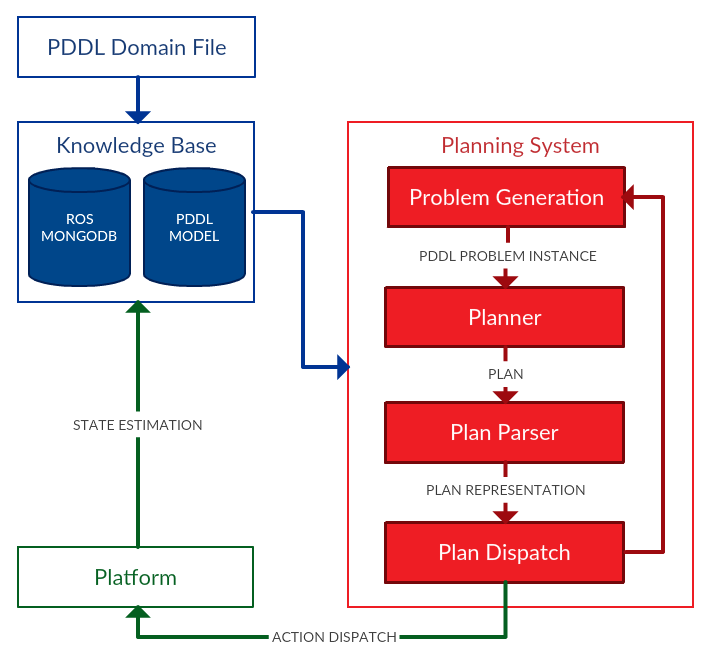
\includegraphics[scale=0.4]{images/overview.png}
	\caption{ROSPlan architecture (image taken from \url{http://kcl-planning.github.io/ROSPlan/documentation/})}
\end{figure} 

\noindent The Knowledge Base stores both the problem domain and problem instance, along with any information to support the planning and stored in a ROS MongoDB. The KB can be updated with ROS messages and queried on-line.
\newpage
\noindent The Planning System:
\begin{enumerate}
\item Fetch information from the KB and generates the PDDL problem file.
\item Call the planner and process the output
\item Dispatches the plan through ROS messages.
\end{enumerate}  
It can also handle replanning due to action failure or plan invalidation. The plan responsible for the planner output parsing and dispatch is the \textbf{Plan Parser}. Two default plan parser are included in ROSPlan: one for sequential plans and another for Esterel program. \\
The first provides a list of action dispatch messages. The second stores the plan as an Esterel language program\footnote{\url{https://en.wikipedia.org/wiki/Esterel}}, that is represented as a DOT graph. \\

\noindent The standard language and planner in ROSPlan are PDDL 2.1 and POPF\cite{coles2010forward},%\cite{popf}, 
that accepts only domains with temporal constraints and no uncertainty. 
Anyway, is it possible to replace the planner, the problem generation and the plan dispatch by simply providing your implementation of this modules.\\
This was also our case since to integrate the work of this thesis with the ROSPlan architecture some modification, in collaboration with the authors, was necessary. We will talk more about later.

\chapter{System Overview}\label{sec:system}
In this chapter I will present the system infrastructure.\\
\newline

\noindent The main objective of this work is the generation of robust condition plans that deals with uncertainty in the problem representation.\\
This approach consist of interpret the output of a planner and generate the correspondent PNP.\\
This PNP is robust with respect to action failure, as it incorporate sensing actions that helps the robot to discern cases from cases.
The architecture presents two layers, each of which will be discussed in the following:
\begin{itemize}
\item \textbf{the Translator}. This module interprets the output of the planner and translate it into a Conditional Plan.
\item \textbf{the Generator}. Generates the actual PNP from a Conditional Plan representation.
\end{itemize}
Each high level action is represented as C++ atomic function, and the PNP is executed using the PNP execution engine.

\section{Conditional Plan Representation}\label{cp_representation}
A conditional plan is a plan that includes also observations.
This lead to plan with branches, where a branch represent an action outcome that depends on a property (the observation) that holds true (or not). \\
These observations are used to handle uncertainty that arises from the lack of knowledge. The uncertainty is handled at execution time, rather than a planning time, where undesirable events are more likely to appear.\\
The conditioning on actions can remove threats by separate the contexts, through the use of conditional or sensing operators.
These operators help the robot to disambiguate the context and must be always executable. At a low level, this means that the robot is equipped with some perception routines that helps him characterise the scenario.\\
Some could be:
\begin{itemize}
\item Face Detection: to detect if there is a person standing in front of him.
\item Speech Recognition: to understand human needs.
\item Semantic Mapping: to reason about spatial context.
\end{itemize} 
If one can predict the type of failure that may arise during the execution of an action, and model them in the domain, the produced plan is more likely to be continuously executed, with no or limited needs for replanning.\\
The explicit representation used for conditional plan is the following:
\begin{verbatim}
plan{
    <state_id>[label=<state_label>,action=<action>]
                 ...
    "<state_0>" -> "<state_1>"
    "<state_1>" [A] -> "<state_2>" ; "<state_1>" [not A] -> "<state_N>"
                     ...
}
\end{verbatim}\\
Where are first listed the state with their id and description, and then all the transitions. Transitions could be either deterministic or conditional, where the conditions, enclosed between the square brackets, are boolean predicates evaluated at runtime.

\noindent As this certainly increase the robustness of the computed plans, at the same time the search space increase tremendously. Consider For instance an state space of observable properties of dimension $N$. If we consider only boolean evaluations, the complete space increases as $O(2^N)$. So we must be very careful when dealing with this kind of representation. The discussion of intelligent search algorithms that can exploit, for instance, the structure of the problem are behind the discussion of this thesis. Instead, I will talk about the translation of this kind of plans into an executable PNP.


\section{Translator Module}
The translator module maintain an internal representation of the conditional plan described in \ref{cp_representation} and is responsible for calling PNPgen, that will generate the actual PNP.
The subset of languages/planners chosen in this thesis are PDDL, KPDDL and ROSPlan PDDL.\\
In the following section I will discuss, for each of the chosen formalism, how the translation works.  

\subsection{PDDL Translator}
PDDL, as stated in \ref{pddl}, is the standard de facto for AI planning. \\
PDDL vers. 2.1 doesn't have natively syntax constructs that allow conditioning on action effects and this lead to the born of different extension, like KPDDL.
%In PDDL however, one can use the "\textbf{when}" in the action description effect to discriminate cases at %planning time. 
Thus, PDDL planners usually generate total ordered plans.\\ 
Also in this case, the chosen planner (Fast-Forward) provides us an ordered list of actions. It estimate an heuristic by relaxing the problem and apply to it a graphplan algorithm.
This kind of solution are interpreted as linear plans. 
The algorithm that realize the translation is listed below:
%The author consider also others planning systems for conformant, contingent and probabilistic planning, but these are not considered in this work.
\newline 
\scalebox{0.85}{
\begin{algorithm}[H]
\caption{ConditionalPlan translation from FF output Algorithm}
\SetKwInOut{Input}{Input}
\SetKwInOut{Output}{Output}
\SetKwProg{Fn}{Function}{}{}
\Input{$\pi$: the PDDL description of the plan}
\KwData{$v_s$: a list of strings}
\Output{$\pi_{cp}$: A Condition Plan}

open $\pi$\;
\While{$\pi$ not eof}{
		\If{line $\neq$ empty and valid}{
			$preProcess($line$)$\;
			$v_s \leftarrow$ line\; 
		}
		$getLine($line$)$;
}

initialize $\pi_{cp}$\;
\For{i less than $sizeof(v_s)$}{
	$s = makeState($i-th element of $v_s)$\;
	i-th element of $\pi_{cp} = s$\;
	$addOutcome(s$, i-th+1 element of $\pi_{cp})$\;
}
\Return  $\pi_{cp}$\;
\Fn{ $makeState(state\_description)$}{
state\_name = $findName(state\_description)$\;
state\_action = $findAction(state\_description)$\;
\ForEach{parameter in state\_description}{
 $add($state,$parameter)$\;
}
\Return state\;
}

\end{algorithm}}\\

\noindent The algorithm reads action by action from the FF output. The states are generated incrementally from each of this line and linked one after the other. \\
\newline
\noindent Even if the generated plan is not conditional, we decide to incorporate PDDL for multiple reasons.\\ 
First of all, we want to show the actual needs for conditional plans in the study cases.
Second, PDDL is the most diffused planning language. Since one of the primary intents of this work is to provide a general tool for PNP generation, it is clear that we cannot ignore it.\\
Many formalisms derive from PDDL, so this class could represent a starting point to implement other translators for different PDDL extensions. \\
Furthermore, the generation of this kind of plans is very fast (linear in time in the number of actions) and composing different linear plans is possible to obtain more complex behaviours.

\newpage
\subsection{KPDDL Translator}
Linear plans are good to model simple cases, but the real world is full of non-determinism and uncertainty.
KPDDL introduces a special construct to the classical PDDL structure that could model sensing effects, and allows formalising sensing actions. This helps the agent to disambiguate between two epistemic states: the one in which the sensed property holds and the case in which not.\\
\newline

\scalebox{0.80}{
\begin{algorithm}[H]
\caption{ConditionalPlan translation from KPlanner output Algorithm}
\SetKwInOut{Input}{Input}
\SetKwInOut{Output}{Output}
\SetKwProg{Fn}{Function}{}{}
\Input{$\pi$: the KPDDL description of the plan}
\KwData{	$v_s$: a list of strings}
\Output{$\pi_{cp}$: A Condition Plan}

open $\pi$\;
\While{$\pi$ not eof and line not empty}{
	$v_s \leftarrow$ line\;
}

$\pi_{cp} \leftarrow makeState($ first of $v_s$)\;
$\pi_{cp} \leftarrow makeState($ last of $v_s$)\;
\ForEach{element $e$ of $v_s \neq$ (first,last)\\}{
	s = $makeState(e)$\;
	$\pi_{cp} \leftarrow makeState(e)$\;
}
\Return $\pi_{cp}$\;
$ $\\
\Fn{ $makeState(state\_description)$}{
state\_name = $findName(state\_description)$\;
state\_action = $findAction(state\_description)$\;
\eIf{condition in state\_description}{
	\While{$observation \leftarrow findObservation(state\_description)$}
	{$addConditionalOutcome(state,observation)$\;}
}
{$addDeterministicOutcome(state)$\;}

\Return state\;
}

\end{algorithm}}

\newpage
\subsection{ROSPlan Translator}\label{sec:digraph_transl}
ROSPlan offers different representation for plans, as discussed in \ref{sec:rosplan}. \\
Nonetheless it was necessary to use a different planner respect to the one provided, namely CLG\cite{clg}\footnote{\url{http://www.ai.upf.edu/software/clg-contingent-planner}}. 
CLG stand for Closed-Loop Greedy planner. \\
This planner rely on a slightly modified version of PDDL which introduce a syntax structure to action effects, \textbf{:observe}, that it is used to define sensing actions, in a very similar way to KPDDL.\\
The description of the problem P, which represent a non-deterministic search problem in belief space, is translated into a non-deterministic problem X(P) in state space by the CLG suite.\\
CLG Planner then accepts P and solves it using X(P) for keeping track of the beliefs and a strengthening relaxation X+(P) to choose which action to apply next.
The relaxation is a classical planning problem that provides an informed heuristic
estimator which embeds the sensing. \\
The solution is semantically interpreted as a digraph (a directed graph), which is represented as:
\begin{verbatim}
    digraph plan_#N{
        state1[ label= "sense_action" ];
        state2[ label= "action_param1_param2" ];
                     ...
        "state1" -> "state2" [ label="obs" ];
        "state1" -> "stateN" [ label="(not(obs))" ];
                     ...
    }
\end{verbatim}
Each state is presented with the corresponding actions, and actions with multiple outcomes have multiple entries along with the property to observe (enclosed between square brackets).
This plan is published on a ROS topic and processed by our node, as we will discuss later.\\
The algorithm is similar to the ones of KPDDL and PDDL:\\
\scalebox{0.8}{
\begin{algorithm}[H]
\caption{ConditionalPlan translation from CLG output}
\SetKwInOut{Input}{Input}
\SetKwInOut{Output}{Output}
\SetKwProg{Fn}{Function}{}{}
\Input{$\pi$: the digraph description}
\KwData{	$v_p$: a list of pair}
\Output{$\pi_{cp}$: A Condition Plan}

open $\pi$\;
\While{line == state\_description }{
	id = $readId(line)$\;	
	action = $readAction(line)$\;
	$v_p \leftarrow \{id,action\}$\;
}

initialize $\pi_{cp}$\;
\ForEach{p in $v_p$}{
	state\_name = first of p\;
	state\_action = second of p\;
	i-th element of $\pi_{cp}$ = state\;
}

\While{line $\neq$ eof}{
	source = $findSource(line)$\;
	destination = $findDestination(line)$\;
	\eIf{line contains observation}{
		observation  = $findObservation(line)$\;
	}{
		observation = ""\;
	}
	\eIf{observation $\neq$ ""}{
		addConditionalOutcome(observation,$findPosition(\pi_{cp},destination)$)\;
	}{
		addDeterministicOutcome($findPosition(\pi_{cp},destination)$)\;
	}
	
	$getLine(line)$\;
}
$\pi_{cp} \leftarrow addGoal()$\;
\Return $\pi_{cp}$\;

\end{algorithm}}\\
\newline
\noindent Notice that the planner doesn't specify a goal state, so we add a goal after each leaf for safety of execution.
The solution and the correspondent translation are computed almost instantaneously, thanks to CLG heuristic, making it possible to run the complete algorithm on-line on a ROS node. 

\section{Generator Module}\label{sec:generator}
\subsection{PNPgen: A Conditional Planning Extension}
Summarizing, the languages formalism induce the following solutions:
\begin{itemize}
\item \textbf{PDDL (FF planner)}: produce a linear plan.
\item \textbf{PDDL (CLG Planner)}: produce a tree. 
\item \textbf{KPDDL (KPlanner)}: produce a direct graph.
\end{itemize}
In order to achieve our results, it was necessary to extend PNPgen module to consider also conditional plans.\\
This means, in particular, to realize a graph search on the conditional plan. In fact the generation of the actual PNP, once we have created the conditional plan, is common for every formalisms.\\


\noindent In the next section I will discuss the algorithm that is responsible for PNPs generation.
\subsection{the Generation Algorithm}
The algorithm responsible for the generation of the PNP performs a graph expansion using the conditional plan representation kept by the correspondent translator class.\\
The simplest case is the one of the standard PDDL domain, in which the algorithm recursively expands the serial sequence of states. In fact, for each, there is only one successor and no observation. \\

\scalebox{0.8}{
\begin{algorithm}[H]
\SetKwInOut{Input}{Input}
\SetKwInOut{Output}{Output}
\Input{$\pi$: the conditional plan,\\
 	   $s_i$: $\pi$ initial state}
\Output{$\pi_c$: PNP generated from the plan}
\eIf{$\pi$ has next}{
	$p_1 \leftarrow$ generatePlace($s_i$)\;
	addPlace($\pi_c$,$p_1$)\;
	recursive call on ($\pi$.next, $p_1$)\;
}{return\;}
\caption{Generate Serial Plans Algorithm}
\end{algorithm}
}\\

\noindent More interesting is the case of the plans with observations, as showed in algorithm \ref{cond_gen}.\\
In order to be sure that every node is visited only once, and thus to avoid dangerous loops in the generation procedure, we maintain a stack of the visited nodes.
Each time, we take the top of this stack, check if it is a final state or has outgoing edges, and expand it.
If it hasn't outcomes, we add a final state and continue with the search. Otherwise, for each edge, we check if the corresponding destination is already in the visited map. If this is the case, we connect it with the current state and close the loop. Otherwise we expand it and create a new branch. \\

\noindent In the next chapter I will show some examples and results to demonstrate the approach. \\
In particular, I will characterize the input/output of each problem and provide a sketch for a possible optimal solution.

%\newpage
\scalebox{0.8}{
\begin{algorithm}[H]
\label{cond_gen}
\SetKwInOut{Input}{Input}
\SetKwInOut{Output}{Output}
\Input{$\pi$: a Conditional Plan,\\
 	   $s_f$: $\pi$ final state\\
 	   $M_{SA}$: a Map between state-action and outcomes}
\KwData{$M_V$: a Map of the visited places\\
        $SS$: a Stack containing the places to explore\\
        $v_o$: a list of possible action outcomes}
\Output{$\pi_c$: PNP generated from a Conditional Plan}
 %\KwResult{how to write algorithm with \LaTeX2e }
  $curr\_state \leftarrow \pi.first\_state$\; 
  $\pi_c \leftarrow addCondition(init)$\;
  $M_V \leftarrow insert(curr\_state)$\;
  $SS \leftarrow push(curr\_state)$\;
 \While{(SS $\neq$ 0)}{
  curr\_state = top of SS\;
  $SS.pop()$\;
  action = $M_{SA}[curr\_state]$\;
  \If{(action == "" and curr\_state $\neq s_f$ )}{
  	continue\;  
  }
  $v_o \leftarrow M_{SA}[curr\_state].outcomes$\;
  \If{$v_o == 0$}{
  	$addFinalState(\pi_c)$\;
  	continue\;
  }
  $addAction(\pi_c,action,current\_state)$\;
  \ForEach{element $e$ of $v_o$\\}
  {
  	$succ\_state = successor(e)$\;
  	$obs = observation(e)$\;
  	\eIf{$M_V[succ\_state] == 0$}
  	{$addBranch(\pi_c, obs)$\;
  	 $SS.push(succ\_state)$\;
  	 $M_V.add(succ\_state)$\;}
  	{$addTransitionBack(\pi_c,obs)$\;}
  }
 }
 \caption{PNPgen from Conditional Plan}
\end{algorithm}}\\

\chapter{Use Cases}\label{sec:use_cases}
In this section I will characterize some examples, describing the whole process from the problem definition to the plan generation.\\ In order to do so I will start from the motivating example introduced in section \ref{sec:motivating}.

%\section{Motivating Example: Implementation}
\section{from PDDL to PNP}
\noindent PDDL was meant to express the "physics" of a domain, and could not represent the epistemic state of an agent.\\
The plan is generated and then executed with "eyes closed". The advantage of this kind of approach is that is very fast, but it could easily fail due to mismatch between the planned plan and the real world.

\newpage
\subsection{Example 1: COACHES}
I will present a solution in PDDL (ver. 1.2) to the example presented in \ref{sec:motivating}.
%PDDL is the standard "de facto" for the specification of planning problems. 
We must then characterise objects, predicates, actions, initial and final states.\\
I used FF\cite{hoffmann:nebel:jair-01}\footnote{\url{https://fai.cs.uni-saarland.de/hoffmann/ff.html}}(ver. 2.3)  planner to check the satisfiability of the problem and to solve it.
For the sake of clarity, in the domain description I will consider only the agent $h2$ of the example. \\

\noindent For the predicates we have:
\begin{verbatim}
(:predicates
            ;robot and person properties
            (person ?x) (robot ?x)
            (at-robot ?x) (at-person ?x)
            (close-to ?x)(wait ?x)(bags-loaded ?x)

            ;needs represents the person necessity
            (needs-help ?x) (needs-WC ?x) (needs-obj ?x)
            (needs-food ?x) (needs-clothes ?x)(satisfied ?x)

            ;desire predicates used to disambiguate which food/cloth
            (desire-italian ?x) (desire-chinese ?x)
            (desire-sportive ?x) (desire-fashion ?x)

            ;locations predicates
            (SHOP ?x) (entrance ?x) (WC ?x) (market ?x)
            (sportive-clothes ?x) (fashion-clothes ?x)
            (chinese-restaurant ?x) (italian-restaurant ?x)

)
\end{verbatim}
Beside from predicates that model environmental properties, we notice the ones that (tries to) describe agents state. 
\noindent For what concern actions, I will not list them all, but I rather focus on the ones that are supposed to be sensing actions:
\begin{verbatim}
(:action sense-person
                      :parameters ( ?r ?p)
                      :precondition (and(person ?p)(robot ?r)(wait ?r))
                      :effect (not(wait ?r))
)
\end{verbatim}

\begin{verbatim}
(:action ask_clothes
           :parameters ( ?r ?p ?x)
           :precondition (and (person ?p)(robot ?r)(close-to ?p))
           :effect (and
                        (needs-clothes ?p)
                        (when
                              (and (at-person ?x)(sportive-clothes ?x))
                              (desire-sportive ?p)
                        )
                        (when
                              (and (at-person ?x)(fashion-clothes ?x))
                              (desire-fashion ?p)
                        )
                   )
)
\end{verbatim}

\begin{verbatim}
(:action ask_food
             :parameters ( ?r ?p ?x)
             :precondition (and (person ?p)(robot ?r)(close-to ?p)(at-person ?x))
             :effect (and
                          (needs-food ?p)
                          (when
                                (italian-restaurant ?x)
                                (desire-italian ?p)
                          )
                          (when
                                (chinese-restaurant ?x)
                                (desire-chinese ?p)
                          )
                     )
)
\end{verbatim}

\begin{verbatim}
(:action ask_object 
             :parameters ( ?r ?p ?x)
             :precondition (and (person ?p)(robot ?r)(close-to ?p)(at-person ?x)(market ?x))
             :effect (needs-obj ?p)
)
\end{verbatim}

\noindent It is clear from the specifications that they are not real sensing actions, as we have previously defined.\\ 
In fact, in standard PDDL, the construct "\textbf{when}" is the only one that allow a simple form of conditioning on actions effects. 
All the information must be known at planning time in order to compute a solution and there isn't the possibility of specifying actions with non-deterministic effects.

\noindent The objects are:
\begin{verbatim}
  (:objects shop1 shop2 shop3
          shop4 shop5 shop6
          entr1 entr2
          food clothes obj
          WC help none
          r h2
  )
\end{verbatim}
\noindent where $\{food, clothes, obj, WC, help, none\}$ models the Z variables presented in \ref{sec:motivating}.\\
\noindent We can then characterize the initial and final state as:
\begin{verbatim}
(:init (robot r)(person h2)
       (wait r) (desire-fashion h2)
	   (at-robot shop4) (at-person shop2)
       (entrance entr1)(entrance entr2)
       (SHOP shop1)(SHOP shop2)(SHOP shop3)
       (SHOP shop4)(SHOP shop5)(SHOP shop6)
       (market shop1)(WC shop3)
       (sportive-clothes shop2)(fashion-clothes shop4)
       (chinese-restaurant shop5)(italian-restaurant shop6)
)
(:goal (satisfied h2) )
\end{verbatim}
\noindent Given this domain and this problem instance, where the "\textit{desire-fashion h2}" predicate is explicitly indicated in the initial state, the output of the FF planner is:
\begin{verbatim}
ff: parsing domain file
domain 'COACHES' defined
 ... done.
ff: parsing problem file
problem 'H2-PLAN' defined
 ... done.    

ff: found legal plan as follows

step    0: SENSE-PERSON R H2
        1: MOVE SHOP4 SHOP2 R
        2: APPROACH-PERSON H2 SHOP2
        3: ASK_CLOTHES R H2 SHOP1
        4: BRINGTO R H2 SHOP2 SHOP4
        5: ADVERTISE-FASHION SHOP4 H2
        6: CHECK_SATISFACTION H2
\end{verbatim}
\noindent In this scenario, we can imagine an infrastructure with a planning system responsible of the generation of the problem instances and a module responsible for gathering the informations (through sensors and physical interfaces) and that manage fluents. This module, for instance, would be the one responsible for the Knowledge Base updates so to justify the presence of  "\textit{desire-fashion h2}" ground in the initial state description.\\

\noindent Once the solution is computed and stored in a file, the PDDL translator fills its internal structure to represent the plan and subsequently expose it to PNPgen. The correspondent translation is the following:

\begin{verbatim}
plan{ 
 n_states=7
 0[label=0,actions=sense-person_r_h2]
 1[label=1,actions=move_shop4_shop2_r]
 2[label=2,actions=approach-person_h2_shop2]
 3[label=3,actions=ask_clothes_r_h2_shop1]
 4[label=4,actions=bringto_r_h2_shop2_shop4]
 5[label=5,actions=advertise-fashion_shop4_h2]
 6[label=6,actions=check_satisfaction_h2]

 "0" -> "1"
 "1" -> "2"
 "2" -> "3"
 "3" -> "4"
 "4" -> "5"
 "5" -> "6"
}
\end{verbatim}

\begin{figure}[H]
	\centering
	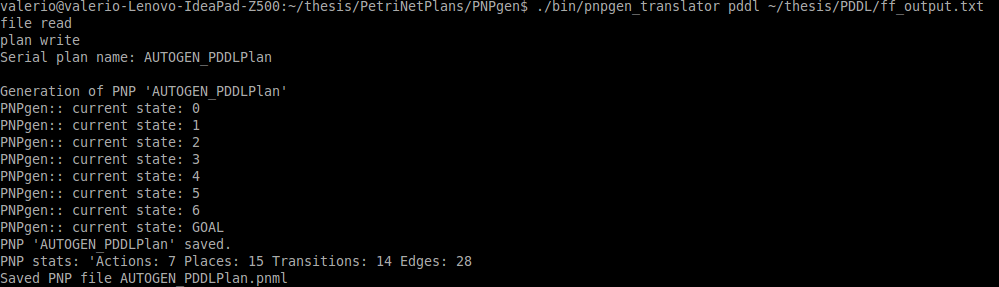
\includegraphics[scale=0.4]{images/pddl_coaches.png}
	\caption{PNPgen generates the PNP from FF output.}
\end{figure}

\noindent When the PNP is generated, it could be visualized and manipulated using Jarp. The correspondent PNP in showed in \ref{fig:pddl_coaches}.\\ 
The whole process, translation+generation, take place in 0,005s (average time). The planning runs in only 0,007s.\\ All the results are obtained using the linux command \textbf{time}\footnote{\url{https://linux.die.net/man/1/time}}.  

\newpage
\begin{figure}[H]
	\centering
	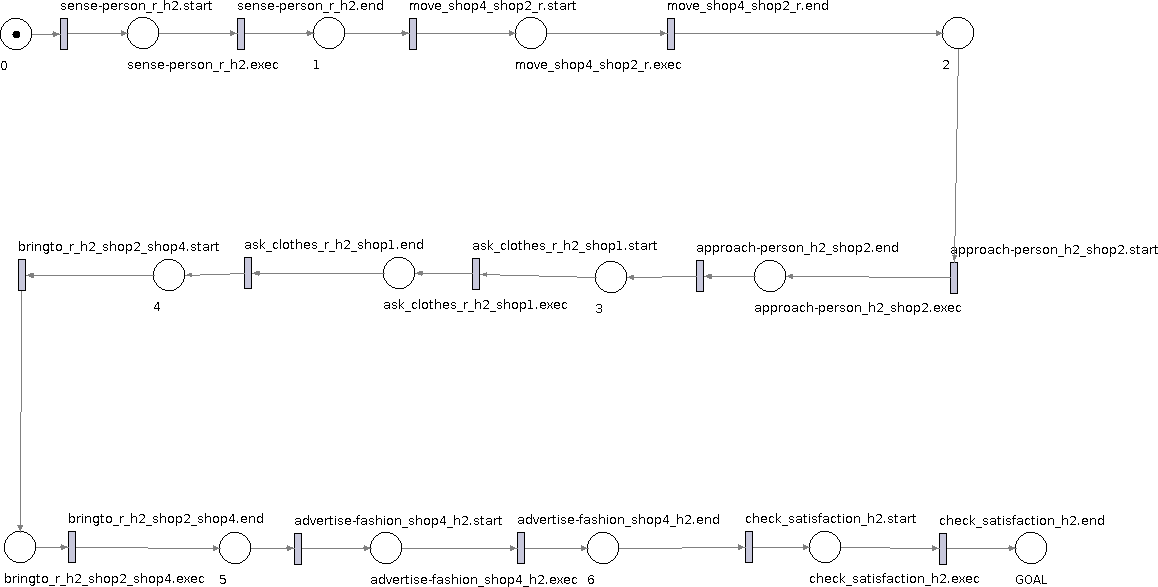
\includegraphics[scale=0.48, angle=270, trim=60mm 0mm 0mm 0mm]{images/coaches_pddl.png}
	\caption{the PNP generated from the coaches PDDL domain. Notice that we had to modify the PNP for a better visualization.}
	\label{fig:pddl_coaches}
\end{figure}
\newpage

\subsection{Example 2: Gripper Problem}
The problem consists in a robot with two hands, moving balls from a room A to a room B. The size of the problem is expressed terms of balls to move from one room to another. We show that doubling the problem size the generation algorithm double its runtime, i.e. the algorithm is linear in the problem size.\\
This is demonstrated in the following table:
\begin{figure}[H]
	\centering
	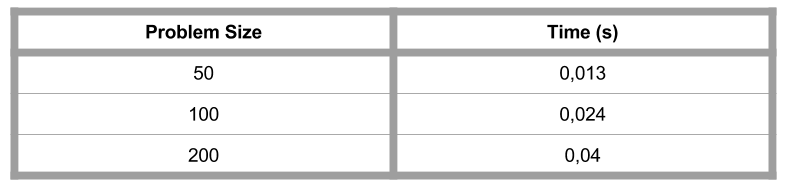
\includegraphics[scale=0.48]{images/gripper_pddl.png}
	\caption{the time for PNPgen to run for an increasing size problem.}
	\label{fig:gripper_pddl}
\end{figure}
\noindent Where the time is the average among five algorithms runs. Obviously also PNPs double their sizes, as we can see from the generation stats:
\begin{enumerate}
\item \textbf{50 balls:} Actions: 149 Places: 299 Transitions: 298 Edges: 596.
\item \textbf{100 balls:} Actions: 299 Places: 599 Transitions: 598 Edges: 1196.
\item \textbf{200 balls:} Actions: 599 Places: 1199 Transitions: 1198 Edges: 2396.
\end{enumerate}

\section{from KPDDL to PNP}
\noindent KPDDL permits to represent conditional plans. The cons reside in the fact that depending on the written domain, the planner could take much time to compute a solution. The author provides the possibility to drive the solution search by the means of a heuristic factor that varies in the range of $[0.0 - 1.0]$, indicating with 0 a breadth-first search while with 1 a depth-first search.\\ 
In any case, this not represents a safe solution for an on-line approach as there are no ways to know if a solution exist (see \ref{sec:analysis}).

\subsection{Example 1: COACHES}
In KPDDL sensing actions could be modelled using the syntactic construct \textbf{:sense}. Most of the predicates, actions and constants remain unchanged with respect to the PDDL case:
\begin{verbatim}

  (:action sense_person
           :parameters ( ?r - robot ?x -location)
           :precondition (sensing ?r)
           :sense (at-person ?x)
  )

  (:action ask_object
           :parameters ( ?p - person )
           :precondition (close-to ?p)
           :sense (needs-obj ?p)
  )

  (:action ask_clothes
           :parameters ( ?p - person )
           :precondition (close-to ?p)
           :sense (needs-clothes ?p)
  )


 (:action ask_food
          :parameters ( ?p - person )
          :precondition (close-to ?p)
          :sense (needs-food ?p)
 )
\end{verbatim}\\
\noindent The substantial difference is that after the execution of such actions the agent knows whether the property sensed by the action is true or false. 
\noindent We can then define the initial state and the goal as following:
\begin{verbatim}
(define
  (problem h2-plan)
  (:domain coaches)
  (:formula-init (and
                     (at-robot shop4)
                     (at-person shop2)
                     (market shop1)
                     (sportive-clothes shop2)
                     (WC shop3)
                     (fashion-clothes shop4)
                     (chinese-restaurant shop5)
                     (italian-restaurant shop6)
                 )
  )

  (:goal
      (satisfied h2)
  )
)
\end{verbatim}
\noindent As we can see, we do not need to model explicitly in the initial state the knowledge about the person needs.\\
\textit{satisfied} is a predicate to indicate a final state and became true after the action \textit{bye}, when the robot as finished to acquire information from the human:

\begin{verbatim}
(:action bye
            :parameters (?p - person)
            :precondition (not (needs-food ?p))
            :effect (satisfied ?p)
)
\end{verbatim}
\noindent As we can see, in this case the property to sense is \textit{needs-food}.
\noindent When given as input to KPlanner, the domain and the problem instance produce the following output:
\begin{verbatim}
INIT: 7
  1 :    approach-person_h2_shop2 --> 2 
  2 :    ask_food_h2 (F) --> 3    ask_food_h2 (T) --> 4 
  3 :    bye_h2 --> 0 
  4 :    bringto_h2_shop2_shop6 --> 5 
  5 :    advertise-italian_h2_shop6 --> 6 
  6 :    bye_h2 --> 0 
  7 :    move_shop4_shop2_r --> 1 
  0 : GOAL
\end{verbatim}\\
\noindent The state description is the conjunction of the properties that holds true in a state.\\ 
Consider, for instance, the state $2, 3, 4$ corresponding to the sensing action \textit{ask\_food} (the ground predicates corresponding to the shops are omitted): 
\begin{verbatim}
  4 = ( at-robot_shop2  at-person_shop2  close-to_h2 )
  5 = ( at-robot_shop2  at-person_shop2  close-to_h2 -needs-food_h2 )
  6 = ( at-robot_shop2  at-person_shop2  close-to_h2 needs-food_h2 )
\end{verbatim}
Here we can notice how the epistemic state changes.\\ 
In particular, after \textit{ask\_food} execution, we can observe two distinct state: one in which \textbf{needs-food\_h2} holds true, and one in which not.

\begin{figure}[H]
	\centering
	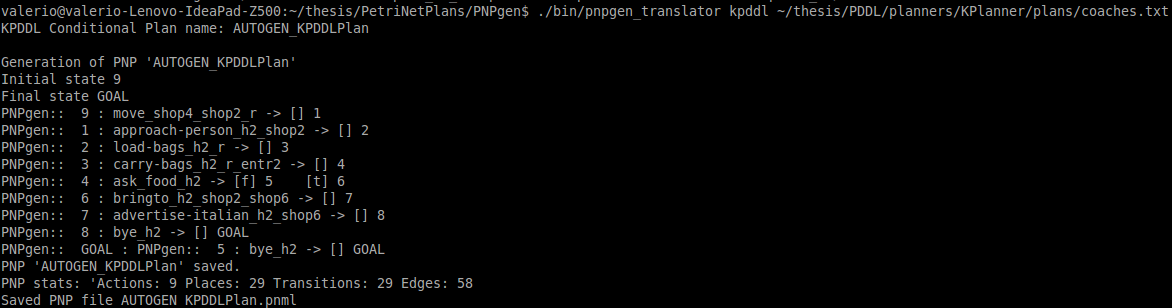
\includegraphics[scale=0.4, trim = 20mm 0mm 0mm 0mm]{images/kpddl_coaches.png}
	\caption{PNPgen generates the PNP from KPlanner output. the observation are enclosed between square brackets.}
\end{figure}

\noindent We translate the solution in our conditional plan representation format. Notice that even the KPlanner output doesn't differ so much from our representation, this is meant to be the same for every considered formalisms (present and future).

\begin{verbatim}
plan{ 

 n_states=8

 0[label=7,actions=move_shop4_shop2_r]
 1[label=1,actions=approach-person_h2_shop2]
 2[label=2,actions=ask_food_h2]
 3[label=3,actions=bye_h2]
 4[label=4,actions=bringto_h2_shop2_shop6]
 5[label=5,actions=advertise-italian_h2_shop6]
 6[label=6,actions=bye_h2]
 7[label=GOAL,actions=]

 "7" -> "1"
 "1" -> "2"
 "2" [f] -> "3" ; "2" [t] -> "4"
 "3" -> "GOAL"
 "4" -> "5"
 "5" -> "6"
 "6" -> "GOAL"

}
\end{verbatim}

\noindent Once represented, we can translate the conditional plan into a PNP.
Action with no conditions are intend to be deterministic, while every time we sense for a property we branch on the boolean result of the action (true or false) as we can see from figure \ref{fig:coaches_kpddlgen}.\\
The planner takes 0.569s on average to run given this problem instance, most of these spent in the search.  
The translation+generation takes only 0.008s time to run. We will compare this results with the ones of the next example.
 
\newpage
\begin{figure}[H]
	\centering
	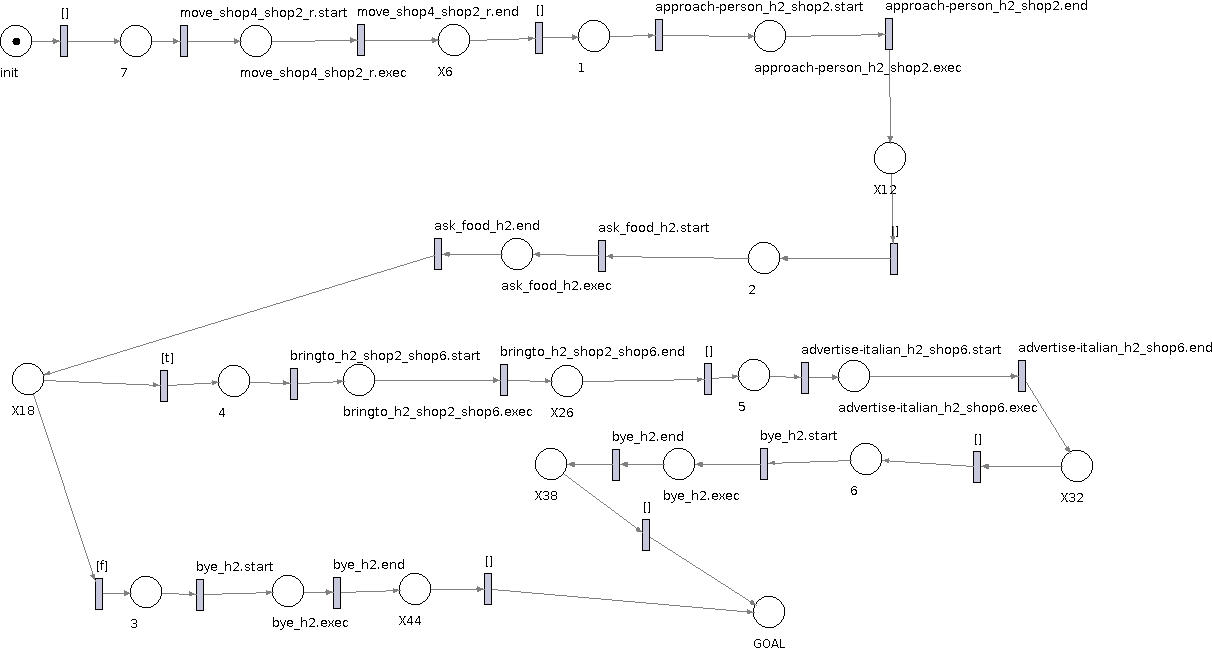
\includegraphics[scale=0.5, angle=270, trim=50mm 0mm 0mm 50mm]{images/coaches_kpddl.png}
	\caption{the PNP generated from the coaches KPDDL domain. Notice that we had to modify the PNP for a better visualization.}
	\label{fig:coaches_kpddlgen}
\end{figure}
\newpage

\subsection{Example 2: COACHES enhanced}
As counterexample, consider the following domain in which we have modified the bye action and we ask the agent to sense for two properties:
\begin{verbatim}
(:action bye
            :parameters (?p - person)
            :precondition (   and
                              (not (needs-obj ?p))
                              (not (needs-food ?p))
                          )
            :effect (satisfied ?p)
)
\end{verbatim}
\noindent The conditional plan correspondent to the computed solution is the following:
\begin{verbatim}
plan{ 

 n_states=12

 0[label=11,actions=move_shop4_shop2_r]
 1[label=1,actions=approach-person_h2_shop2]
 2[label=2,actions=ask_object_h2]
 3[label=3,actions=ask_food_h2]
 4[label=4,actions=bye_h2]
 5[label=5,actions=bringto_h2_shop2_shop6]
 6[label=6,actions=advertise-italian_h2_shop6]
 7[label=7,actions=bye_h2]
 8[label=8,actions=bringto_h2_shop2_shop1]
 9[label=9,actions=advertise-objects_shop1_h2]
 10[label=10,actions=bringto_h2_shop1_shop2]
 11[label=GOAL,actions=]

 "11" -> "1"
 "1" -> "2"
 "2" [f] -> "3" ; "2" [t] -> "8"
 "3" [f] -> "4" ; "3" [t] -> "5"
 "4" -> "GOAL"
 "5" -> "6"
 "6" -> "7"
 "7" -> "GOAL"
 "8" -> "9"
 "9" -> "10"
 "10" -> "3"

}
\end{verbatim}
As we can see is significantly more complex than the previous, as we can also see from the correspondent PNP depicted in \ref{fig:kpddl_ex2}.\\
Such complex PNPs are very time consuming to be manually constructed and error prone. However, we can notice that doubling the number of epistemic variables, the time for the planner to run increases exponentially from 0.569s to 23,8252s! The run time of our system however remain almost the same (from 0,008s to 0,009).
It is clear that if we double the epistemic states, the planner runs indefinitely.

\newpage
\begin{figure}[H]
	\centering
	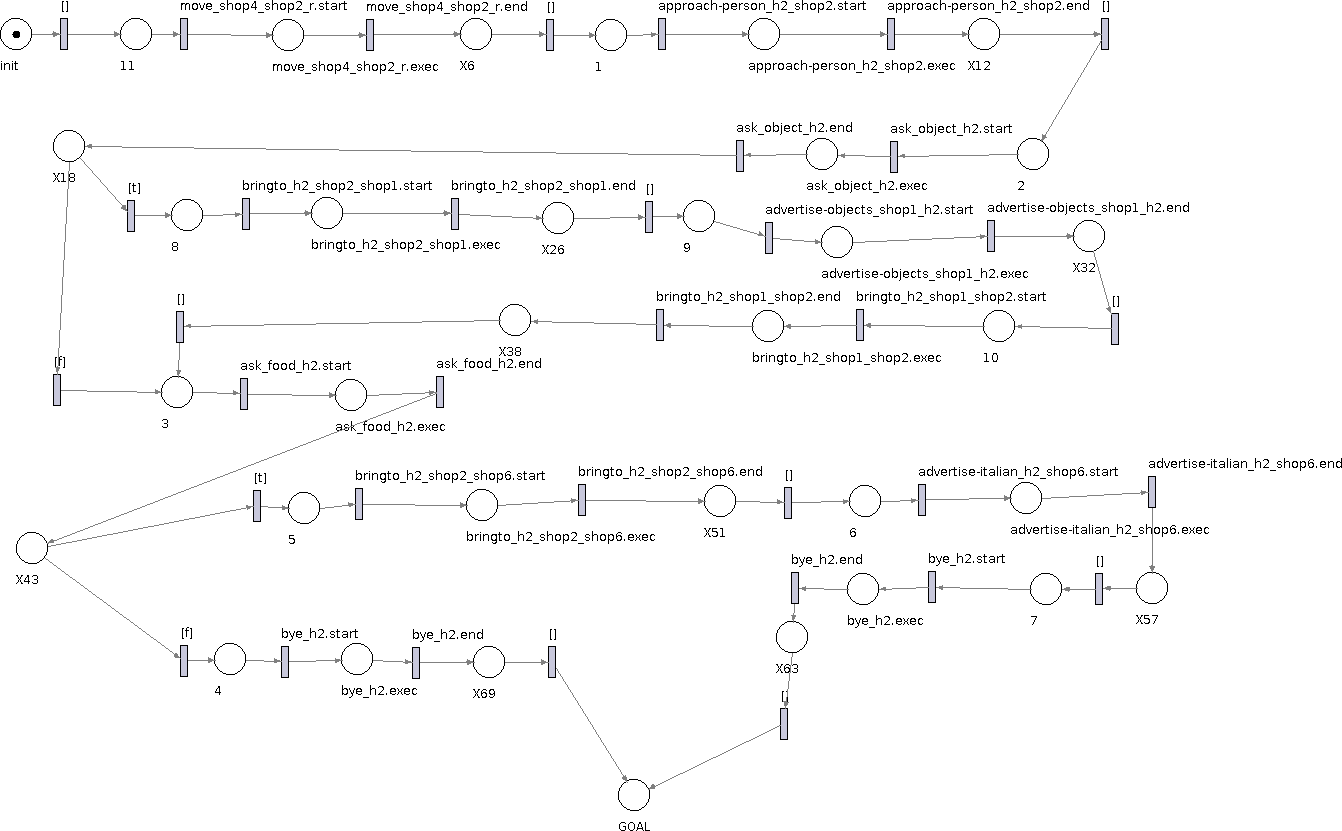
\includegraphics[scale=0.5, angle=270, trim=73mm 0mm 0mm -80mm]{images/kpddl_ex2.png}
	\caption{the PNP generated from the modified coaches KPDDL domain. Notice that we had to modify the PNP for a better visualization.}
	\label{fig:kpddl_ex2}
\end{figure}
\newpage

\section{from ROSPlan PDDL to PNP}
\noindent ROSPlan represents the most prominent solution for an on-line approach.
The used planner, CLG, has a very intelligent heuristic that can present almost instantaneously a solution, when present, or communicate that this not exist. 
The ROSPlan framework is perfectly integrated into ROS and, due to its modularity, it can be extended to consider other formalisms (like we have done for this work).\\

\noindent The infrastructure provides a safe way to handle planning failures, since even when a solution is not found in the first place, it can replan a certain number of times based on a tunable parameter.\\
This comes in handy since if the PNP execution fails, we have a second level of redundancy to make sure that the robot doesn't suddenly stop. \\
The integration between ROSPlan and PNP is an ongoing work and I will discuss possible future implementations in the next chapter.

\subsection{Example 1: simple COACHES}
This is a simplified version of the coaches example, in which we inspect only the person position.
We must introduce a slightly different version of PDDL, similar to KPDDL, that is used in the ROSPlan Framework.\\
As in KPDDL, in this case PDDL is extended with introduction of the \textbf{:observe} construct for action effects, used to define sensing actions.\\
For instance, a sensing action has the following form:
\begin{verbatim}
  (:action sense_person
                       :parameters (?x -location)
                       :precondition (at-robot ?x)
                       :observe (at-person ?x)
  )
\end{verbatim}
Beside from the \textit{observe} construct, we must provide the problem specification with the following expression:
\begin{verbatim}
 (oneof
   (at-person shop1)
   (at-person shop2)
   (at-person shop3)
   (at-person shop4)
   (at-person shop5)
   (at-person shop6)
 )
\end{verbatim}
These are necessary for the planner to derive a supplementary heuristic used while searching for the solution. We avoid to present the complete domain as this is essentially the same of the previous sections.\\

\noindent A ROS node serves as interface between ROSPlan and PNPgen. This node actively listens the topic where the plan is published by the planning system. 
\noindent The planning system fetch the PDDL model from the Knowledge Base and generates a problem instance.
After that, he calls the planner and dispatch its output on the topic "\textit{/kcl\_rosplan/plan\_graph}"

\begin{figure}[H]
	\centering
	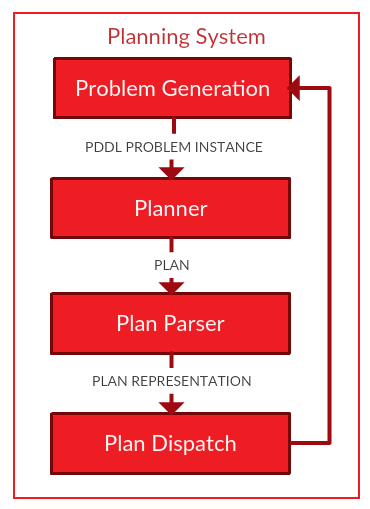
\includegraphics[scale=0.3]{images/dia_system.png}
	\caption{The planning system architecture.}
\end{figure}

\noindent The output is represented as a direct graph, as described in section \ref{sec:digraph_transl}:

\begin{verbatim}
digraph plan_0 {
0[ label="sense_person_shop4" style="fill: #fff; "];
1[ label="move_shop4_shop5_r" style="fill: #fff; "];
2[ label="sense_person_shop5" style="fill: #fff; "];
3[ label="move_shop5_shop3_r" style="fill: #fff; "];
4[ label="sense_person_shop3" style="fill: #fff; "];
5[ label="move_shop3_shop2_r" style="fill: #fff; "];
6[ label="sense_person_shop2" style="fill: #fff; "];
7[ label="move_shop2_shop1_r" style="fill: #fff; "];
8[ label="sense_person_shop1" style="fill: #fff; "];
9[ label="move_shop1_shop6_r" style="fill: #fff; "];
10[ label="approach-person_h2_shop6" style="fill: #fff; "];
11[ label="bye_h2" style="fill: #fff; "];
12[ label="approach-person_h2_shop1" style="fill: #fff; "];
13[ label="bye_h2" style="fill: #fff; "];
14[ label="approach-person_h2_shop2" style="fill: #fff; "];
15[ label="bye_h2" style="fill: #fff; "];
16[ label="approach-person_h2_shop3" style="fill: #fff; "];
17[ label="bye_h2" style="fill: #fff; "];
18[ label="approach-person_h2_shop5" style="fill: #fff; "];
19[ label="bye_h2" style="fill: #fff; "];
20[ label="approach-person_h2_shop4" style="fill: #fff; "];
21[ label="bye_h2" style="fill: #fff; "];
"0" -> "20" [ label="at-person shop4" ];
"0" -> "1" [ label="(not (at-person shop4))" ];
"1" -> "2"
"2" -> "18" [ label="at-person shop5" ];
"2" -> "3" [ label="(not (at-person shop5))" ];
"3" -> "4"
"4" -> "16" [ label="at-person shop3" ];
"4" -> "5" [ label="(not (at-person shop3))" ];
"5" -> "6"
"6" -> "14" [ label="at-person shop2" ];
"6" -> "7" [ label="(not (at-person shop2))" ];
"7" -> "8"
"8" -> "12" [ label="at-person shop1" ];
"8" -> "9" [ label="(not (at-person shop1))" ];
"9" -> "10"
"10" -> "11"
"12" -> "13"
"14" -> "15"
"16" -> "17"
"18" -> "19"
"20" -> "21"
}
\end{verbatim}

\noindent As soon as a plan is published, the node writes it to a file and calls the PNPgen class responsible for the translation and generation of the actual PNP.\\ 
The following picture depict the connection between our node (\textit{pnp\_rosplan\_interface}) and the rest of the architecture:

\begin{figure}[htbp]
	\centering
	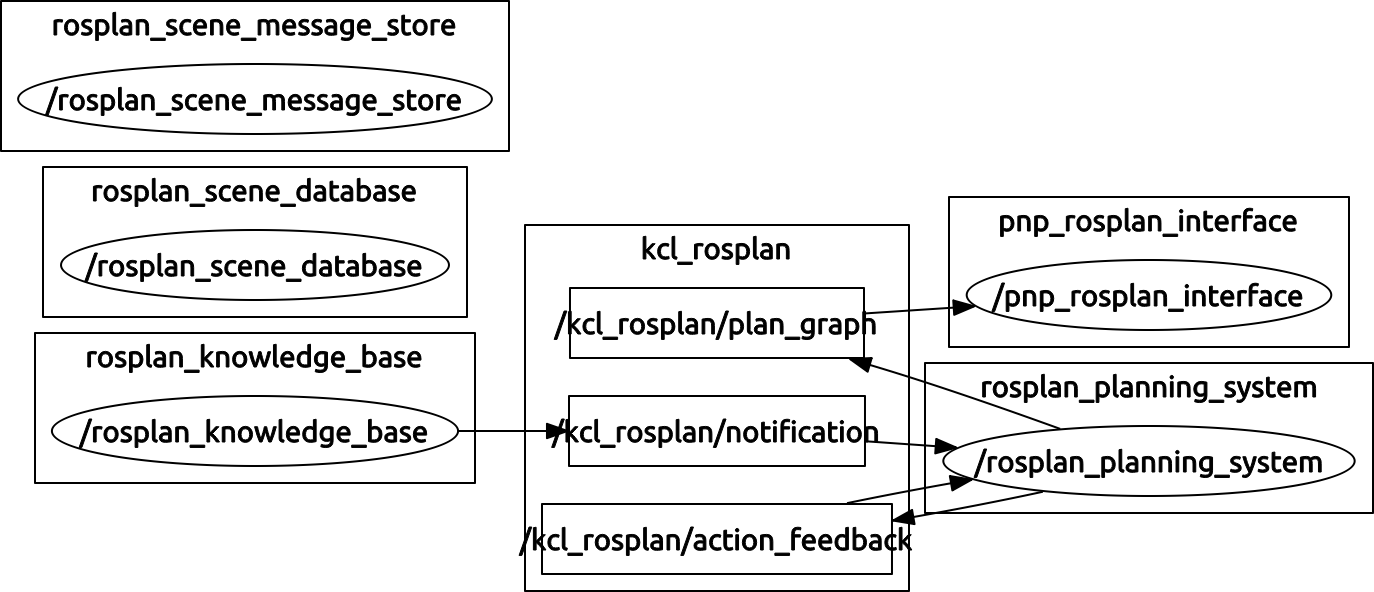
\includegraphics[scale=0.3]{images/rospnp.png}
	\caption{A snapshot of the nodes used to translate a digraph into a PNP.}
\end{figure}

\noindent You will find a portion of the correspondent PNP in the next page.\\
\newpage
\begin{figure}[H]
	\centering
	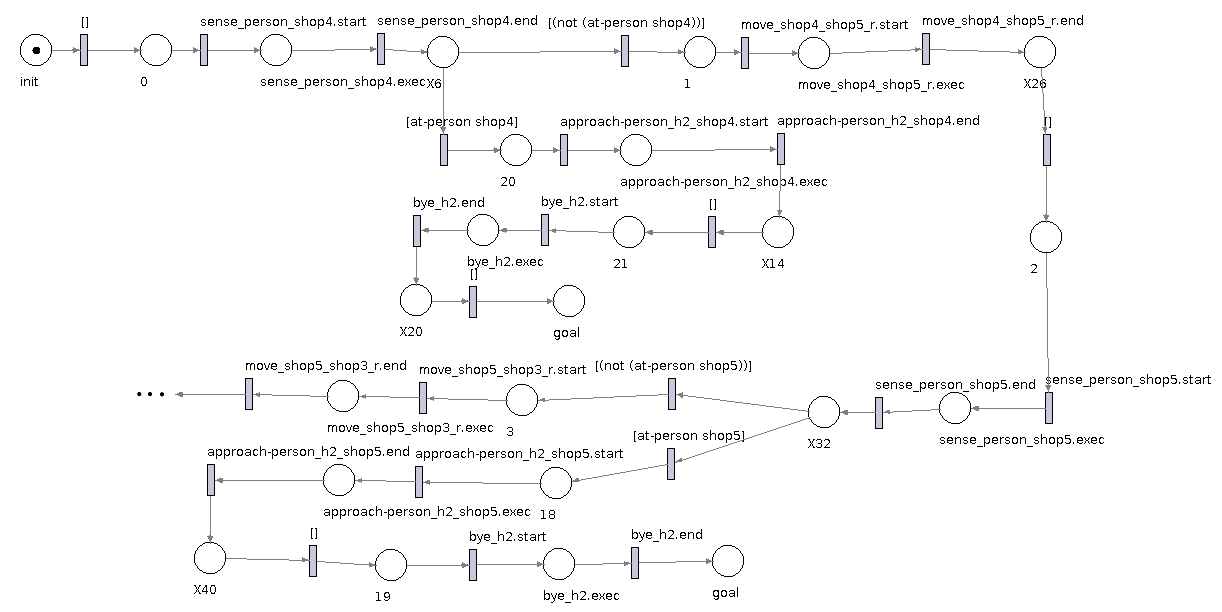
\includegraphics[scale=0.4]{images/rosplan_coaches1.png}
	\caption{a portion of the PNP generated from the ROSPlan Digraph. Notice that we had to move some places/transitions for a better visualization.}
\end{figure}

%PNP stats: 'Actions: 22 Places: 68 Transitions: 67 Edges: 134

\subsection{Example 2: COACHES complete}
This is the complete coaches example, as presented in the previous sections. Namely, we try to infer also the person needs using the following sensing action:
\begin{verbatim}
  (:action ask
    :parameters ( ?p - person ?x - desire)
    :precondition (close-to ?p)
    :observe (needs ?x)
  )
\end{verbatim} 
\noindent The predicate \textit{needs} can take five values: 	obj, food, clothes, WC and help.
As before, we must specify the possible outcomes in the initial state:
\begin{verbatim}
  (:init (and
             (at-robot shop4)
             (oneof
               (at-person shop1)
               (at-person shop2)
               (at-person shop3)
               (at-person shop4)
               (at-person shop5)
               (at-person shop6)
             )
             (oneof
               (needs obj)
               (needs food)
               (needs clothes)
               (needs help)
               (needs WC)
             )
         )
  )
\end{verbatim}

%PNP stats: 'Actions: 70 Places: 212 Transitions: 211 Edges: 422
\noindent We do not show the complete PNP since it is too big to fit in a page. Consider that for this case there are 211 places and 422 edges. As we can see from the image \ref{fig:rosplan_ex2}, the generated PNP is complete in the sense that can represent the epistemic knowledge of the robot and the generation happens almost instantaneously. This example concludes our analysis.

\begin{figure}[H]
	\centering
	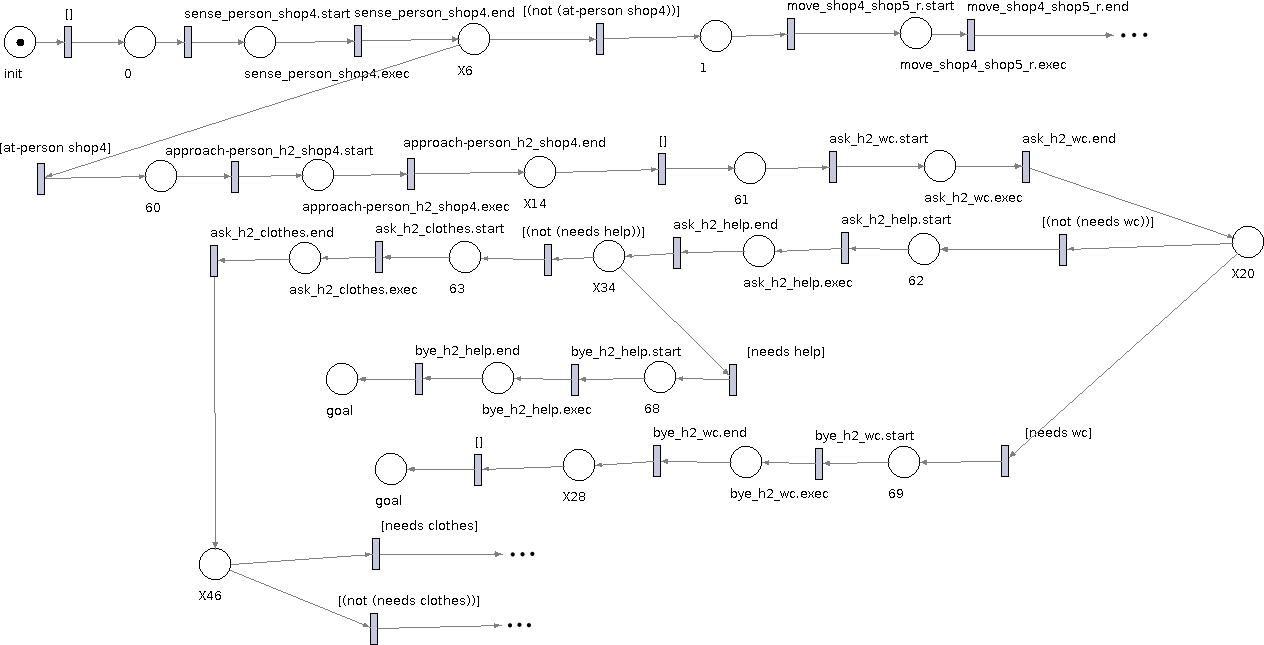
\includegraphics[scale=0.5,angle=270, trim=50mm 0mm 0mm 0mm]{images/rosplan_coaches2.png}
	\caption{a small portion of the PNP generated from the complete coaches domain. Notice that we had to modify the PNP for a better visualization.}
	\label{fig:rosplan_ex2}
\end{figure}


%\subsection{Example 3: Wumpus}

\chapter{Conclusion}\label{sec:conclusion}
One of the fundamental aspects of moving robots from laboratories to everyday environments is that the interaction with unaware persons should be the most natural and smooth as possible.\\
In fact, a robot that "freeze" during an interaction or that could not response actively to the external stimuli is very far from the definition of social.\\
In this work we have discussed an approach that tries to take advantage of the expressivity of some of the languages and formalisms present in the literature to represent, generate and execute conditional plans, i.e. plans that incorporates observations.\\
This kind of plans are robust with respect to action failures since we can represent very complex plans that are otherwise impossible to write "manually".
Using the PNP framework we can easily visualize and eventually modify a plan.\\
Furthermore, we have demonstrated the integration of our work with an infrastructure that runs on-line on the robot and how promising this approach is. We are indeed collaborating with ROSPlan\ref{sec:rosplan} authors to extend further this work. 


\section{Future Development}
There are some things still missing in our framework that can be considered for future implementations.\\
For instance, it is evident the lack of a graphical interface.
It is clear that if we want to expand our work considering more formalisms, a tool that automatically selects one or another based on desired properties becomes fundamental.

\begin{figure}[H]
	\centering
	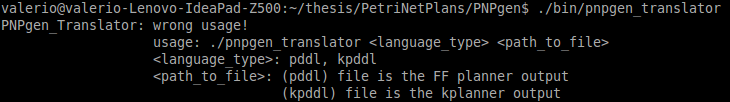
\includegraphics[scale=0.5]{images/pddltransl.png}
	\caption{the current interface to generate PNPs from (K)PDDL.}
\end{figure}

\noindent Talking about formalisms to be added

%A robot must be capable of discerning cases in which an interaction is desirable and cases in which is not. Like in the simple case of a "welcome robot", it is important that the robot says "hi" when a person shows in front of him but it must also take into account the fact that a person could appear in front of him multiple times. 
%Another important but maybe trickier case is to equip the robot with the capability of understanding the mood of the person and than react consequently. Although this could be seen as a fictional case, since is impossible at the moment even for the most complex cognitive robot to understand emotions, there are some simple cases that could be treated. The goal, in this case, is not to reproduce a perfect model of the human mind state and how it could react to some sorts of events, but rather discover some patterns that could lead to undesirable outcomes. For instance, a person could be busy with its work and the interference of the robot, when is not helpful in the context of the human task, could be perceived as noise. Thus is important to maintain a representation of the person daily routines and enrich this when is possible with the information that comes from the social interactions that occurs from time to time between the two. If we are interested in developing robots strictly social, we cannot leave aside the emotional aspect of the interaction. 


\begin{itemize}
\item Add More Formalisms -- PDDL extensions in the translation
\item Planner selection/study
\item from Boolean Evaluation to an Higher Logic
\item Merging plans
\item ER rules
\end{itemize}


\bibliographystyle{plain}
\bibliography{biblio.bib}


\end{document}
